\documentclass[a4paper,12pt]{article}%

\usepackage{amsmath}
\usepackage{amsfonts}
\usepackage{amssymb}
\usepackage{graphicx}
\usepackage[czech]{babel} %Cestina
\usepackage[cp1250]{inputenc}%hacky, carky
\usepackage{hyperref}
\usepackage{wasysym} %kvuli znacce prumeru
\usepackage{multicol} %umozni vkladat vicesloupcove bloky

%okraje stranky
\usepackage{geometry}
 \geometry{
 a4paper,
 %total={210mm,297mm},
 left=20mm,
 right=20mm,
 top=20mm,
 bottom=20mm,
 }


%-------------------------------------------

\begin{document}

\setcounter{tocdepth}{1} %V obsahu pouze nazvy uloh
\tableofcontents


%\section{\texorpdfstring{Elektrick� obvody}{Elektricke obvody}}

\subsection{\texorpdfstring{�vod}{Uvod}}
Alespo� ur�it� schopnost n�vrhu elektrick�ho obvod mus� pat�it mezi z�kladn� v�domosti absolventa technick�ho oboru se zam��en�m na elektrotechniku. Elektrick� obvody lze t��dit z mnoha hledisek. Podle pou�it�ch sou��stek je lze rozd�lit nap��klad na aktivn�, tj. ty kter� obsahuj� zdroje energie a pasivn�, tj. ty kter� energii pouze spot�ebov�vaj�. D�le pak na vysokofrekven�n�, n�zkofrekven�n�, line�rn�, neline�rn� atd.

V tomto cvi�en� je pozornost zam��ena na pasivn� d�li�e nap�t�. A�koliv se jedn� o velice jednoduch� stavebn� blok elektrick�ch obvod�, pat�� tak� mezi ty nejpou��van�j��. Prakticky v ��dn�m elektronick�m obvodu je nelze vynechat. Lze se s nimi setkat ve zp�tn�ch vazb�ch zesilova��, p�i nastavov�n� pracovn�ch bod� tranzistor�, lze jimi impedan�n� p�izp�sobovat v�stupy zdroj� nap�t�, pou��vaj� se v sond�ch osciloskop� atd.

\subsubsection{\texorpdfstring{D�li� nap�t�}{Delic napeti}}

Pasivn� d�li� nap�t� je realizov�n dv�ma rezistory. Vstupn� nap�jec� nap�t� je rozd�leno v podob� �bytk� nap�t� v pom�ru dan�m hodnotami obou rezistor�. V�stupn� nap�t� se obvykle z�sk�v� pouze z rezistoru se spole�nou zem� s nap�jec�m zdrojem. Vztah pro d�l�c� pom�r nezat�en�ho d�li�e lze z�skat z Ohmova z�kona:

\begin{equation}
U_{20} = R_2 \cdot I = R_2 \cdot \frac{U_1}{R_1 + R_2} \Longrightarrow \frac{U_{20}}{U_1}=\frac{R_2}{R_1 + R_2}=\frac{1}{1 + \frac{R_1}{R_2}}
\label{eq:elObv:vystNapDel}
\end{equation}

Podle Theveninova teor�mu lze spojen� d�li�e nap�t� a nap�ov�ho zdroje nahradit zdrojem nap�t� s nap�t�m $U_{20}$ a s vnit�n�m odporem $R_i$. Vnit�n� odpor n�hradn�ho zdroje je z�sk�n jako odpor mezi v�stupn�mi svorkami po nahrazen� v�ech zdroj� nap�t� v obvodu zkratem. V p��pad� d�li�e jsou pak oba odpory paraleln� a z�sk�v�me vztah:

\begin{equation}
R_i = \frac{R_2 \cdot R_1}{R_1 + R_2}
\label{eq:elObv:vnitrOdpor}
\end{equation}

Uveden� �vahy neplat� jen pro rezistory, ale i pro obecnou impedanci (tj. v d�li�i mohou b�t i reaktance).

\subsubsection{\texorpdfstring{Frekven�n� p�izp�soben�}{Frekvencni prizpusobeni}}

V�stupn� nap�t� $U_2$ odporov�ho d�li�e m��e b�t frekven�n� z�visl� v d�sledku p��tomnosti parazitn�ch reaktanc�. P�i spojov�n� funk�n�ch blok�, jako nap��klad zdroj nap�t� a z�t�, je obvykle t�eba kompenzovat p�edev��m kapacitu z�t�e $C_2$. Pomysln� d�li� nap�t� vznik� mezi vnit�n�m odporem zdroje $R_1$ a odporem z�t�e $R_2$. P�ipojen� kapacita s rostouc� frekvenc� sni�uje v�slednou impedanci z�t�e a nap�t� na z�t�i kles�. Dan� jev lze kompenzovat p�ipojen�m dal��ho kondenz�toru $C_1$ paraleln� k vnit�n�mu odporu zdroje $R_1$. Pro d�l�c� pom�r dan�ho obvodu lze postupn� odvodit:

\begin{equation}
\frac{U_2}{U_1} = \frac{\frac{R_2}{1+j\omega R_2 C_2}}{\frac{R_1}{1+j\omega R_1 C_1} + \frac{R_2}{1+j\omega R_2 C_2}}=\frac{1}{1+\frac{R_1 \cdot (1+j\omega R_2 C_2)}{R_2 \cdot (1+j\omega R_1 C_1)}}
\label{eq:elObv:odvozKompenzace}
\end{equation}

V rovnici (\ref{eq:elObv:odvozKompenzace}) je $\omega = 2\cdot\pi\cdot f$ uhlova frekvence. Z�ejm� bude d�l�c� pom�r frekven�n� nez�visl� za p�edpokladu:
\begin{equation}
\frac{R_1 - \frac{j}{\omega\cdot C_1}}{R_2 - \frac{j}{\omega\cdot C_2}} = K,
\label{eq:elObv:kompenzace}
\end{equation}

\noindent
kde $K$ je ur�it� konstanta. Hodnotu konstanty lze odvodit p�i znalosti jednotliv�ch prvk� obvodu a tento �kol je sou��st� n�sleduj�c�ch cvi�en�. Vnit�n� impedanci n�hradn�ho zdroje nap�t� lze op�t odvodit dle Theveninova teor�mu, ��m� z�sk�me v�echny �ty�i prvky d�li�e paraleln�.

\begin{figure}[h]
  \centering
  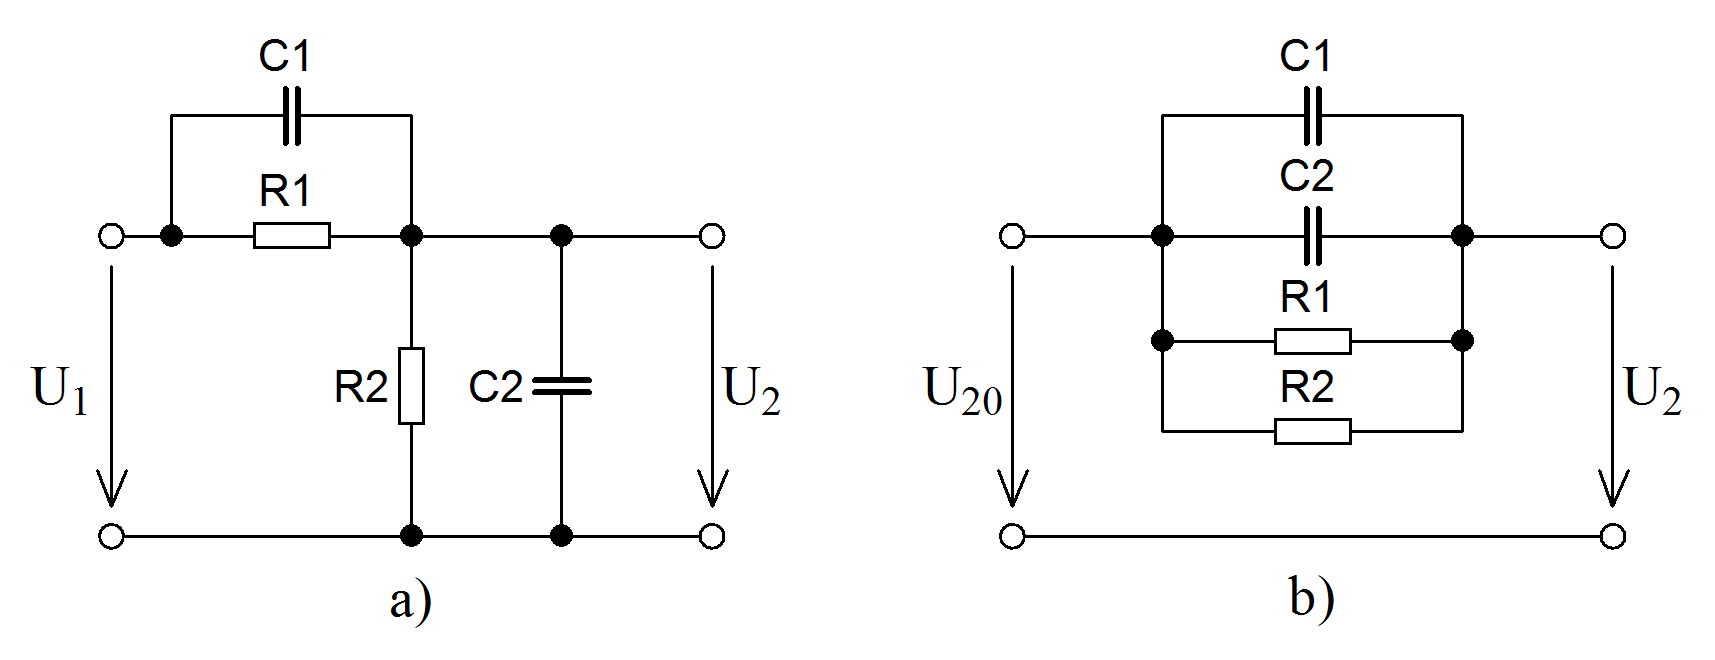
\includegraphics[width=0.8\columnwidth]{el_obvody/teorie}
	\caption{a) frekven�n� kompenzovan� d�li� nap�t�, b) n�hradn� sch�ma zdroje podle Thevenina}
  \label{fig:elObv:teorie}
\end{figure}

%---------------------------------------------
\newpage
\subsection{\texorpdfstring{Frekven�n� p�izp�soben� pasivn�ho d�li�e nap�t�}{Frekvencni prizpusobeni pasivniho delice napeti}}

\subsubsection{\texorpdfstring{�kol m��en�}{Ukol mereni}}
\begin{enumerate}
 \item [a)] Pro dan� frekven�n� nep�izp�soben� d�li� spo�t�te vhodnou hodnotu kapacity v�stupn�ho kondenz�toru, kter�m zajist�te konstantn� d�l�c� pom�r v�stupn�ho nap�t� v �irok�m rozsahu frekvenc�.
 \item [b)] Sv�j n�vrh ov��te m��en�m na p��pravku pro vstupn� nap�t� obd�ln�kov�ho pr�b�hu o frekvenci 500 Hz. Zaznamenejte v�stupn� pr�b�h nap�t� pro p�ekompenzovan�, nedostate�n� kompenzovan� a frekven�n� kompenzovan� d�li� nap�t�.
 \item [c)] Pomoc� osciloskopu a gener�toru sinusov�ho nap�t� zm��te frekven�n� z�vislost v�stupn�ho nap�t� d�li�e po p�ipojen� kondenz�tor� o hodnot�ch 150~nF, 68~nF a 33~nF. M��en� prove�te pro rozsah frekvenc� 100~Hz a� 10~kHz.
\end{enumerate}

Vysv�tlete v z�v�ru rozd�ly mezi frekven�n�mi charakteristikami.

\subsubsection{\texorpdfstring{Sch�ma zapojen�}{Schema zapojeni}}

\begin{figure}[h]
  \centering
  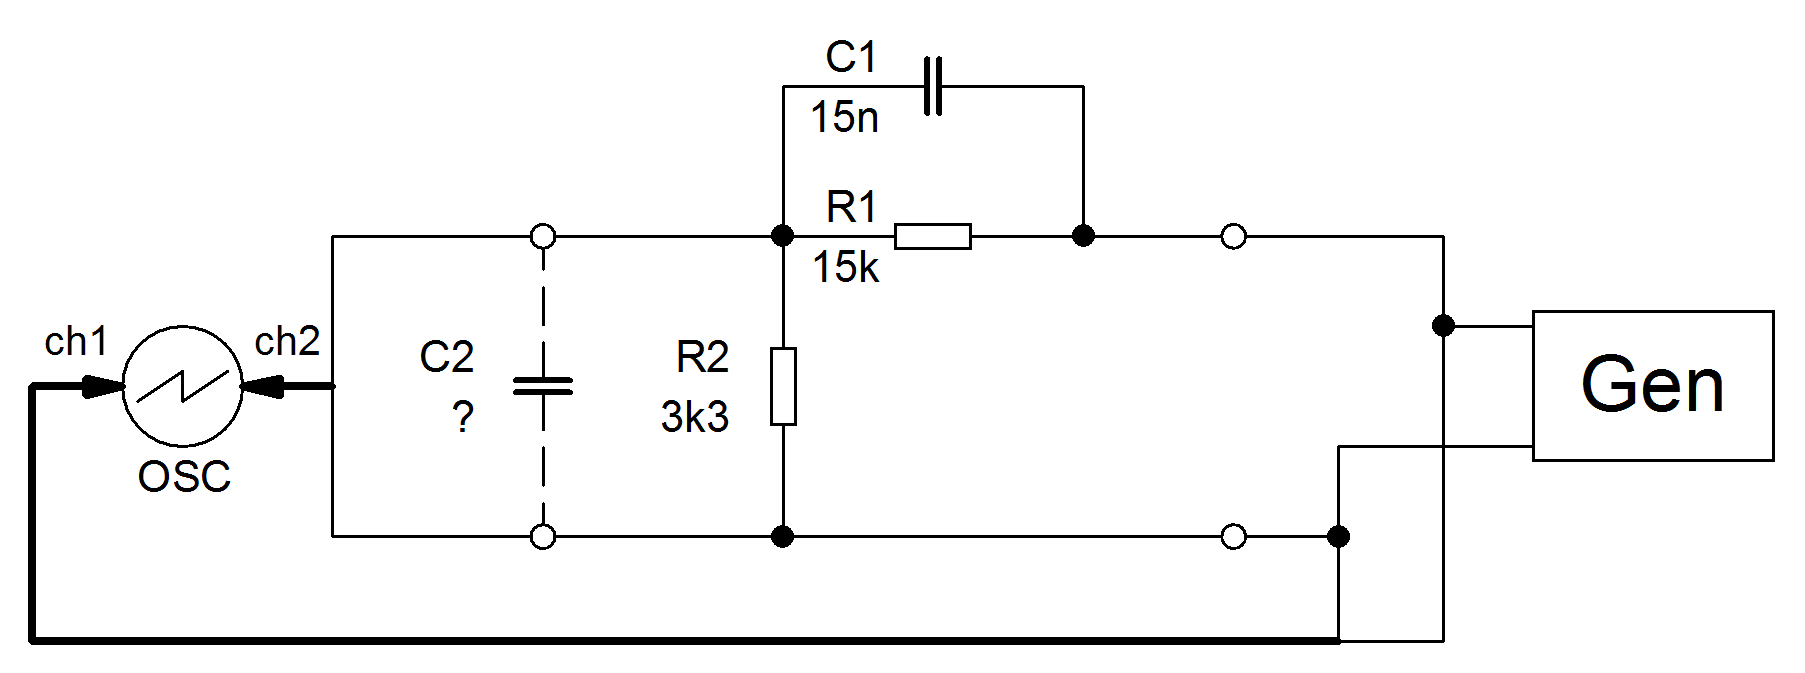
\includegraphics[width=0.75\columnwidth]{el_obvody/elObv}
  \label{fig:elObv:elObv}
\end{figure}

\subsubsection{\texorpdfstring{Postup m��en�}{Postup mereni}}

\begin{description}
 \item [ad a)] �kol lze vy�e�it v�ce zp�soby. Hodnotu vhodn� kapacity lze ur�it v�po�tem �pravou vztahu (\ref{eq:elObv:kompenzace}). Tak z�sk�me p��mo z�vislost mezi jednotliv�mi prvky obvodu d�li�e. Druhou mo�nost� je odzkou�et jednotliv� m��en� vzorky kondenz�tor� p�ipojov�n�m na v�stup d�li�e p�i nap�jen� d�li�e obd�ln�kov�m sign�lem. Pro spr�vnou hodnotu kapacity bude v�stupn� obd�ln�kov� sign�l nezkreslen�. P�i znalosti spr�vn� hodnoty kapacity pak lze dodate�n� snadno vyvodit jej� z�vislost na ostatn�ch prvc�ch obvodu.
 \item [ad b)] P�i ov��ov�n� p�ipojte 1.~kan�l osciloskopu na vstup funk�n�ho gener�toru a 2.~kan�l na v�stup d�li�e. Gener�tor p�ipojte na vstup d�li�e a nastavte na n�m obd�ln�kov� pr�b�h o amplitud� 15~V a frekvenci 500~Hz. Jednotliv� v�stupn� pr�b�hy obd�ln�kov�ch sign�l� zaznamenejte na pam�ov� medium nebo p�ekreslete do se�itu.
 \item [ad c)] Na funk�n�m gener�toru nastavte v�stupn� sinusov� pr�b�h. Zapojen� osciloskopu a gener�toru je stejn� jako v p�edchoz�m �kolu. Pomoc� osciloskopu m��te amplitudu vstupn�ho (nem�n� se) a v�stupn�ho sinusov�ho pr�b�hu. K m��en� amplitudy lze vyu��t rastru st�n�tka osciloskopu nebo kursor� (seznamte se s uveden�mi mo�nostmi). Frekvenci v dan�m rozsahu m��te s logaritmick�m krokem 100~Hz, 200~Hz, 500~Hz, 1~kHz,..., 10~kHz. ��sti rychl�ch zm�n amplitudy v�stupn�ho nap�t� prom��te s men��m krokem. Nap�ov� p�enos ur�ete jako pom�r v�stupn�ho ke vstupn�mu nap�t� a vyneste jej do spole�n�ho grafu pro jednotliv� kondenz�tory p�ipojen� k v�stupu.
\end{description}

%---------------------------------------------
\newpage
\subsection{\texorpdfstring{Impedan�n� p�izp�spoben� vstupu zesilova�e}{Impedancni prizpusobeni vstupu zesilovace}}

\subsubsection{\texorpdfstring{�kol m��en�}{Ukol mereni}}

\begin{enumerate}
 \item [a)] Spojen� gener�toru a kompenzovan�ho d�li�e z p�edchoz� ��sti m��en� uva�ujte jako zdroj obd�ln�kov�ho nap�t� s definovan�m vnit�n�m odporem a s�riovou v�stupn� kapacitou. Vrcholovou hodnotu obd�ln�kov�ho pr�b�hu nap�t� nastavte na gener�toru na 5~V. Ur�ete (a zm��te):
 \begin{itemize}
	\item vrcholovou hodnotu nap�t� napr�zdno - spo�t�te a ov��te osciloskopem nebo voltmetrem p�i nap�jen� stejnosm�rn�m zdrojem 5~V,
	\item vnit�n� (v�stupn�) odpor d�li�e - spo�t�te a ov��te pomoc� m��en� se stejnosm�rn�m zdrojem,
	\item vnit�n� (v�stupn�) s�riovou v�stupn� kapacitu d�li�e - pouze spo�t�te.
 \end{itemize}
Do se�itu zakreslete n�hradn� sch�ma tohoto zdroje s ur�en�mi hodnotami prvk�.
 \item [b)] Upraven� zdroj propojte s p��pravkem tranzistorov�ho zesilova�e s nap�ov�m zes�len�m $A_U=20$~dB. Navrhn�te a zapojte d�li� v b�zov�m obvodu, kter�m nastav�te stejnosm�rn� pracovn� bod tranzistoru a z�rove� definujete vstupn� odpor zesilova�e. Vstupn� odpor zesilova�e zvolte tak, aby po propojen� s d�li�em byl na v�stupu zesilova�e obd�ln�kov� sign�l o vrcholov� hodnot� 4~V, 3~V nebo 2~V (ur�� vedouc� cvi�en�). D�li� nap�jejte z gener�toru obd�ln�kov�m sign�lem o vrcholov� hodnot� 5~V a frekvenci 1~kHz. Zcela jist� bude t�eba upravit paraleln� kapacitu d�li�e, prove�te! Sv�j n�vrh popi�te do se�itu a jeho spr�vnost ov��te m��en�m pomoc� osciloskopu.
\end{enumerate}

\subsubsection{\texorpdfstring{Sch�ma zapojen�}{Schema zapojeni}}

\begin{figure}[h]
  \centering
  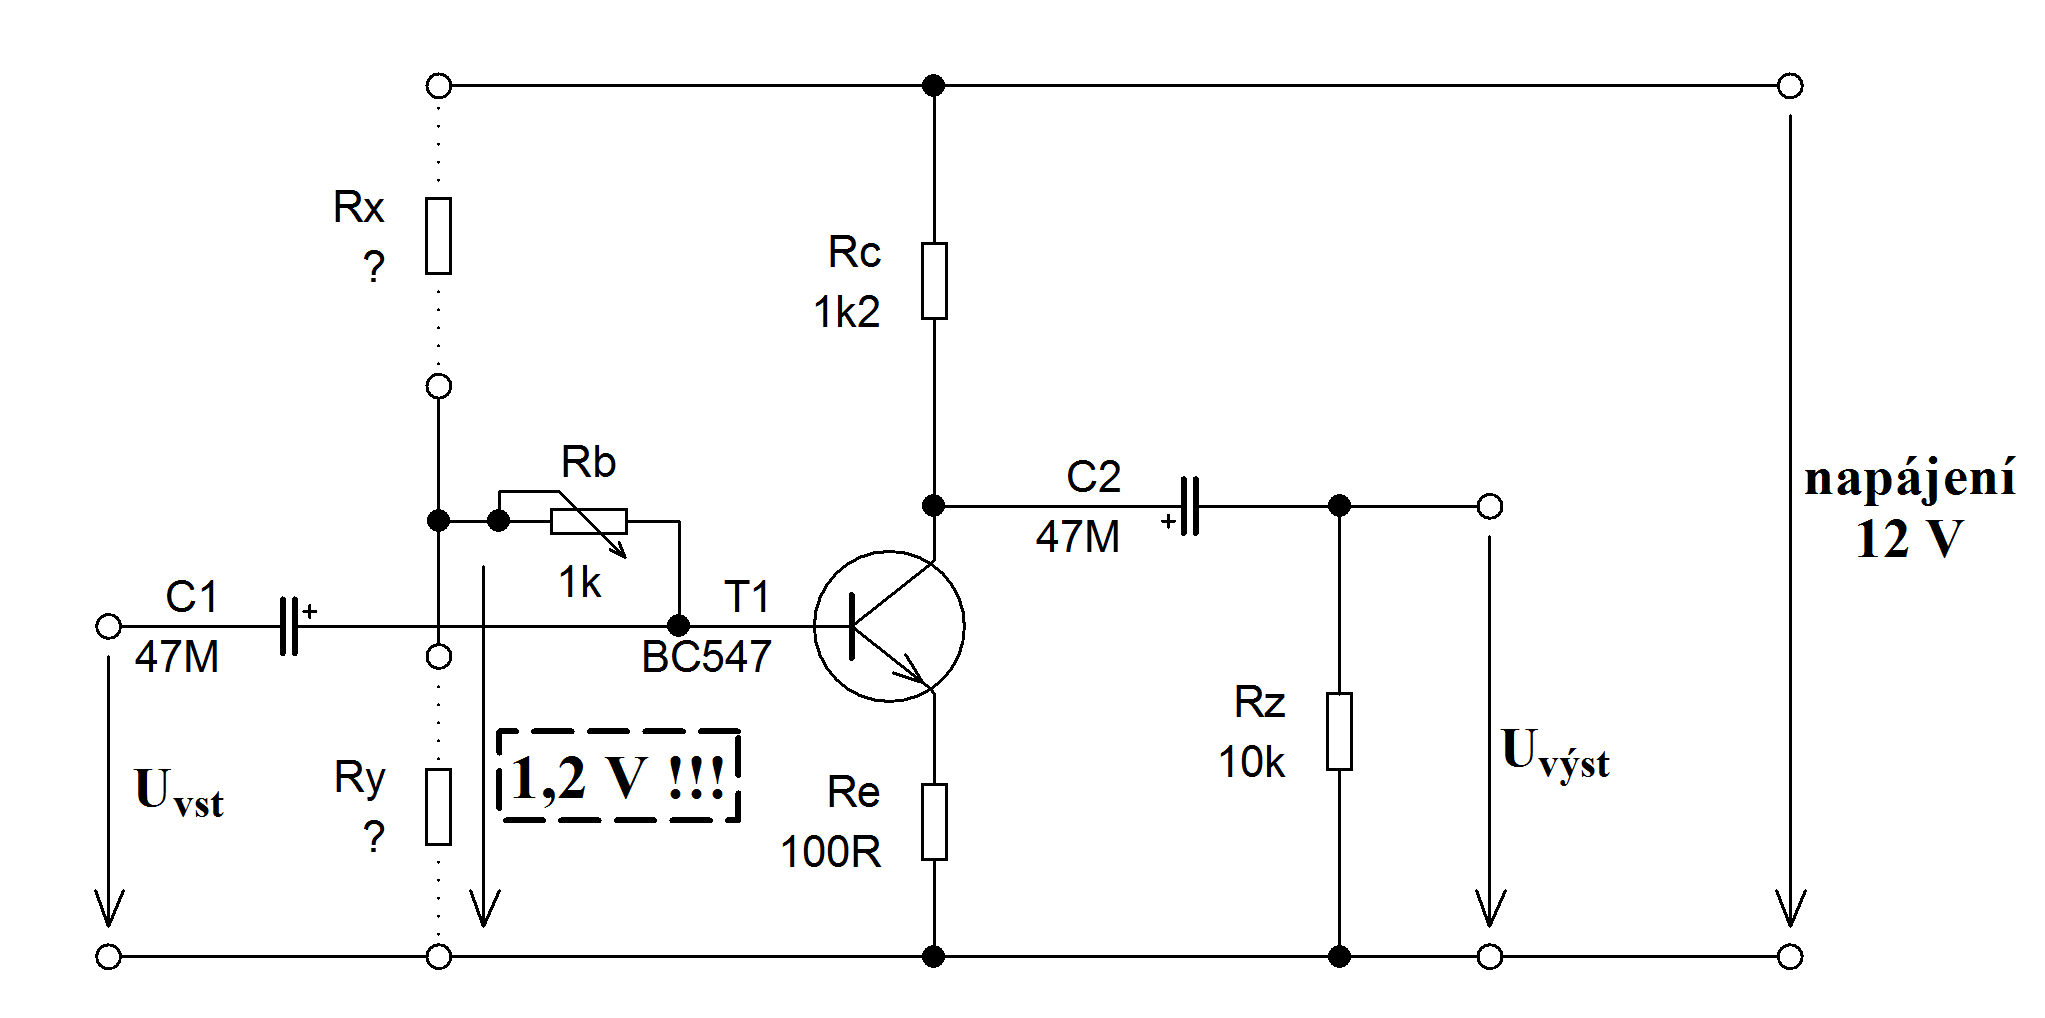
\includegraphics[width=0.9\columnwidth]{el_obvody/zesilovac}
  \label{fig:elObv:zesilovac}
\end{figure}

\subsubsection{\texorpdfstring{Postup m��en�}{Postup mereni}}

\begin{description}
 \item [ad a)] Jeliko� je d�li� frekven�n� kompenzovan�, bude nap�t� napr�zdno $U_0$ d�no bu� pom�rem obou rezistor� nebo obou kapacit (tj. dle p��slu�n�ch vztah�!!!). Ov��en� m��en�m provedeme pro tak�ka nezat�en� d�li�, kdy na jeho v�stup p�ipoj�me voltmetr a vstup budeme nap�jet stejnosm�rn�m zdrojem o nap�t� 5~V. Vnit�n� odpor d�li�e $R_i$ lze spo��tat po zjednodu�en� obvodu podle Theveninova teor�mu. Hodnotu lze ov��it m��en�m n�kolika, av�ak podobn�mi zp�soby. Ten nejjednodu��� spo��v� ve zkratov�n� d�li�e pomoc� amp�rmetru p�i nap�jen� d�li�e stejnosm�rn�m zdrojem. Z amp�rmetru ode�teme zkratov� proud n�hradn�ho zdroje nap�t�. Vnit�n� odpor pak z�sk�me jako pod�l nap�t� napr�zdno a zkratov�ho proudu. Na z�klad� zjednodu�en� obvodu podle Theveninova teor�mu vypo��t�me i v�slednou v�stupn� kapacitu $C_i$ n�hradn�ho zdroje. Ov��en� jej� hodnoty m��en�m je obt�n�. Jej� hodnotu je mo�n� z�skat ze zm��en�ho p�echodn�ho d�je, nebo alespo� p�ibli�n� p�i m��en� na vy���ch frekvenc�ch. V p��pad� z�jmu o m��en� vnit�n� kapacity zdroje pom��e cvi��c�.
 \item [ad b)] Vstupn� odpor zesilova�e zat�� p�ipojen� zdroj sign�lu, v d�sledku �eho� poklesne jeho svorkov� nap�t�. V prvn�m kroku je tedy nutn� ur�it, na jakou hodnotu m��e klesnout vstupn� nap�t�. Pro p��klad uva�ujme, �e v�stupn� �pi�kovou hodnotu nap�t� zesilova�e po�adujeme 6~V. Jeliko� zesilova� zesiluje 10$\times$, pak po�adovan�m vstupn�m nap�t�m je 0,6~V.

Vnit�n� odpor zdroje sign�lu $R_i$ a vstupn� odpor zesilova�e $R_{vst}$ spole�n� vytv��ej� d�li� nap�t� napr�zdno $U_0$ zdroje sign�lu. V�stupn� nap�t� dan�ho d�li�e po�adujeme pr�v� spo�ten�ch 0,6~V. Ze vztahu pro v�stupn� nap�t� nezat�en�ho d�li�e vypo��t�me po�adovanou hodnotu vstupn�ho odporu zesilova�e $R_{vst}$. Z�rove� pro jeho hodnotu podle d��ve odvozen�ch pravidel dopo��t�me kapacitu $C_{vst}$ kondenz�toru, kter� mus� b�t p�ipojen na vstup zesilova�e, aby vstupn� nap�t� bylo frekven�n� nez�visl�.

P�i n�vrhu d�li�e nastavuj�c� pracovn� bod tranzistoru zanedbejte odb�r b�zov�ho obvodu. P�edpokl�dejte, �e je d�li� nezat�en� a neuva�ujte ani hodnotu p�ipojen�ho potenciometru Rb, kter� slou�� pouze k dolad�n� v�sledn� hodnoty vstupn�ho odporu. Pro spr�vn� nastaven� pracovn�ho bodu, mus� b�t v�stupn� nap�t� d�li�e rovno \textbf{1,3~V} p�i nap�jen� 15~V. Vnit�n� odpor navrhovan�ho d�li�e je roven po�adovan�mu vstupn�mu odporu zesilova�e. Podle p��slu�n�ch vztah� dopo��tejte hodnoty prvk� Rx a Ry.

Z �ady E12 zvolte nejbli��� hodnoty odpor� a kapacity kompenza�n�ho kondenz�toru. Obvodov� prvky p�ipojte na p��slu�n� svorky p��pravku zesilova�e. Vstup cel�ho obvodu nap�jejte obd�ln�kov�m sign�lem o �pi�kov� hodnot� 5~V a frekvenci 1~kHz. V�stup zesilova�e zobrazte na osciloskopu. Pokud je patrn� zkreslen� hran sign�lu, pokuste se doladit hodnotu vstupn�ho odporu pomoc� potenciometru na p��pravku. Pokud nelze dos�hnout vykompenzovan�ho sign�lu nebo je �pi�kov� hodnota pr�b�hu nap�t� odli�n� (v�ce jak o 0,4~V) od po�adovan�, pak je t�eba n�vrh d�li�e p�ehodnotit.
\end{description}

\subsubsection{\texorpdfstring{Pou�it� materi�l}{Pou�it� materi�l}}
\begin{tabular}{ll}
 1.& Rezistory �ady hodnot E12, 1~k$\Omega$ - 82~k$\Omega$ \\
 2.& Foliov� kondenz�tory, 33~nF, 68~nF, 150~nF \\
 3.& Keramick� kondenz�tory �ady hodnot E12, 10~nF - 330~nF \\
 4.& P��pravek tranzistorov�ho zesilova�e  \\ 
\end{tabular}
%\section{\texorpdfstring{Ide�ln� sou��stky elektronick�ch obvod�}{Idealni soucastky elektronickych obvodu}}

\subsection{\texorpdfstring{�vod}{Uvod}}
P�i n�vrhu elektrick�ch obvod� zpravidla jednotliv� obvodov� prvky pova�ujeme za ide�ln� a vyjma polovodi�ov�ch sou��stek tak� za line�rn�. Toto cvi�en� se zam��uje na popis a chov�n� elektronick�ch obvod� slo�en�ch z pasivn�ch sou��stek, jak�mi jsou rezistor, c�vka a kondenz�tor p�i harmonick�m (sinusov�m) nap�jen�. P�itom p�edpokl�d�me, �e uveden� prvky vykazuj� pouze sv�j hlavn� charakter a neuva�ujeme jejich parazitn� vlastnosti, jako nap��klad svodov� odpor u kondenz�toru nebo odpor vinut� u c�vky.

\subsubsection{\texorpdfstring{Odpor, reaktance, impedance}{Odpor, reaktance, impedance}}

P�i harmonick�m nap�jen� lze pr�b�hy obvodov�ch veli�in popsat f�zorov�m diagramem a vyu��t mo�nost� oper�torov�ho po�tu Steinmetzovy transformace (n�kde i Fourierovy transformace), kter� nahrad� derivace a integrace n�soben�m a d�len�m �lenem $j\omega$. $\omega$ zde m� v�znam �hlov� frekvence zkouman�ho sign�lu. Z�ejm� se tento typ transformace hod� p�edev��m pro anal�zu harmonick�ho ust�len�ho stavu obvodu. T�mto zp�sobem z�sk�me pro ide�ln� obvodov� prvky oper�torov� impedance (odpor, induktivn� reaktance, kapacitn� reaktance), kter� jsou definovan� n�sleduj�c� vztahy:

\begin{equation}
R =\frac{\widehat{U}_R}{\widehat{I}_R}
\label{eq:idSouc:odpor}
\end{equation}

\begin{equation}
\frac{-j}{\omega C} =\frac{\widehat{U}_C}{\widehat{I}_C}
\label{eq:idSouc:kapacita}
\end{equation}

\begin{equation}
j\omega L =\frac{\widehat{U}_L}{\widehat{I}_L}
\label{eq:idSouc:indukcnost}
\end{equation}

Ze vztah� plyne, �e po zobrazen� f�zor� (vektor�, komplexn�ch ��sel) nap�t� a proudu v komplexn� (Gaussov�) rovin� doch�z� u kapacitoru a induktoru mezi ob�ma veli�inami k f�zov�mu posunu o 90$^\circ$. U ide�ln� c�vky (induktor) se proud za nap�t�m zpo��uje o 90$^\circ$, zat�mco u ide�ln�ho kondenz�toru (kapacitor) proud nap�t� o 90$^\circ$ p�edb�h�. D�le je z�ejm� i vliv frekvence, kdy v p��pad� ide�ln� c�vky je reaktance �m�rn� frekvenci, tj. jej� hodnota roste, zat�mco u kondenz�toru reaktance s frekvenc� kles� a to nep��mo �m�rn�.

P�i spojov�n� v�ce prvk� vyu��v�me po��t�n� s komplexn�mi ��sly. Obecn� komplexn� v�sledek naz�v�me impedanc� obvodu a ozna�ujeme j� $\widehat{Z}$. Plat� pro n� stejn� vyj�d�en� jako pro komplexn� ��sla. Nap��klad impedanci s�riov�ho spojen� rezistoru a induktoru lze popasat jako:

\begin{equation}
\widehat{Z} = R+jX_L = R+j\omega L
\label{eq:idSouc:Zkomplex}
\end{equation}

\noindent
nebo

\begin{equation}
\widehat{Z} = \left|Z\right|\cdot e^{j\varphi}
\label{eq:idSouc:Zexp}
\end{equation}

\noindent
Pro �leny v rovnici (\ref{eq:idSouc:Zexp}) plat�:

\begin{equation}
\left|Z\right|= \sqrt{R^2 + (\omega L)^2}
\label{eq:idSouc:absZ}
\end{equation}

\begin{equation}
\varphi= arctg\left(\frac{\omega L}{R}\right)
\label{eq:idSouc:fiZ}
\end{equation}

\subsubsection{\texorpdfstring{F�zorov� diagram}{Fazorovy diagram}}
F�zorov� diagramy jsou vlastn� zobrazen�m hodnot obvodov�ch veli�in v komplexn� rovin�. Diagram mus� v�dy spl�ovat Kirchhoffovy z�kony, proto sou�et v�ech f�zor� proud� v jednom uzlu mus� b�t nula a stejn� tak i sou�et v�ech f�zor� nap�t� jedn� smy�ky (jin�mi slovy, v diagram tyto f�zory mus� tvo�it uzav�en� obrazec). Pokud zn�me hodnoty nap�t�, proud� a f�z� v jednotliv�ch ��stech obvodu, je jedno, kter� f�zor nakresl�me jako prvn�. V ostatn�ch p��padech v�dy za��n�me od f�zoru, kter� je v obvodu nejd�le od nap�jec�ch svorek, tak jako bychom obvod �e�ili postupn�m zjednodu�ov�n�m. D�le m�me mo�nost volby nato�en� re�ln� a imagin�rn� osy v��i cel�mu diagramu. U komplikovan�j��ch obvod� b�v� obvykl� (ne p�edepsan�) u nap�jen� nap�ov�m zdrojem umis�ovat do re�ln� osy f�zor nap�jec�ho nap�t� a p�i nap�jen� zdrojem proudu f�zor nap�jec�ho proudu. U jednoduch�ch zapojen� (1-3 prvky) se do re�ln� osy obvykle umis�uje obvodov� veli�ina, kter� je spole�n� v�em prvk�m.

Po�ad� kreslen� jednotliv�ch f�zor� pro ur�it� obvod ukazuje obr�zek \ref{fig:idSouc:fazDiag}. Pro p�ehlednost jsou odd�leny f�zory nap�t� a proudu. Diagram za��n� vy�e�en�m f�zor� proudu v RC obvodu. Proud rezistorem je v m���tku zakreslen horizont�ln�. Jeliko� nap�t� na paraleln� kombinaci je ob�ma prvk�m spole�n� a ve f�zi s proudem rezistoru, mus� proud kapacitorem p�edb�hat o 90$^\circ$. Sou�et obou f�zor� pak d�v� v�sledn� proud $I$. N�sleduje zakreslen� nap�t� $U_{RC}$ ve f�zi s proudem rezistoru. Nap�t� na c�vce mus� o 90$^\circ$ p�edb�hat v�sledn� proud $I$ a sou�et obou nap�t� d� v�sledn� nap�t� zdroje. Jako posledn� se zakresluj� osy, v��i kter�m se m��� v�echny f�zov� �hly a podle pot�eby se diagram oto�� (p�ekresl�).

\begin{figure}[h]
  \centering
  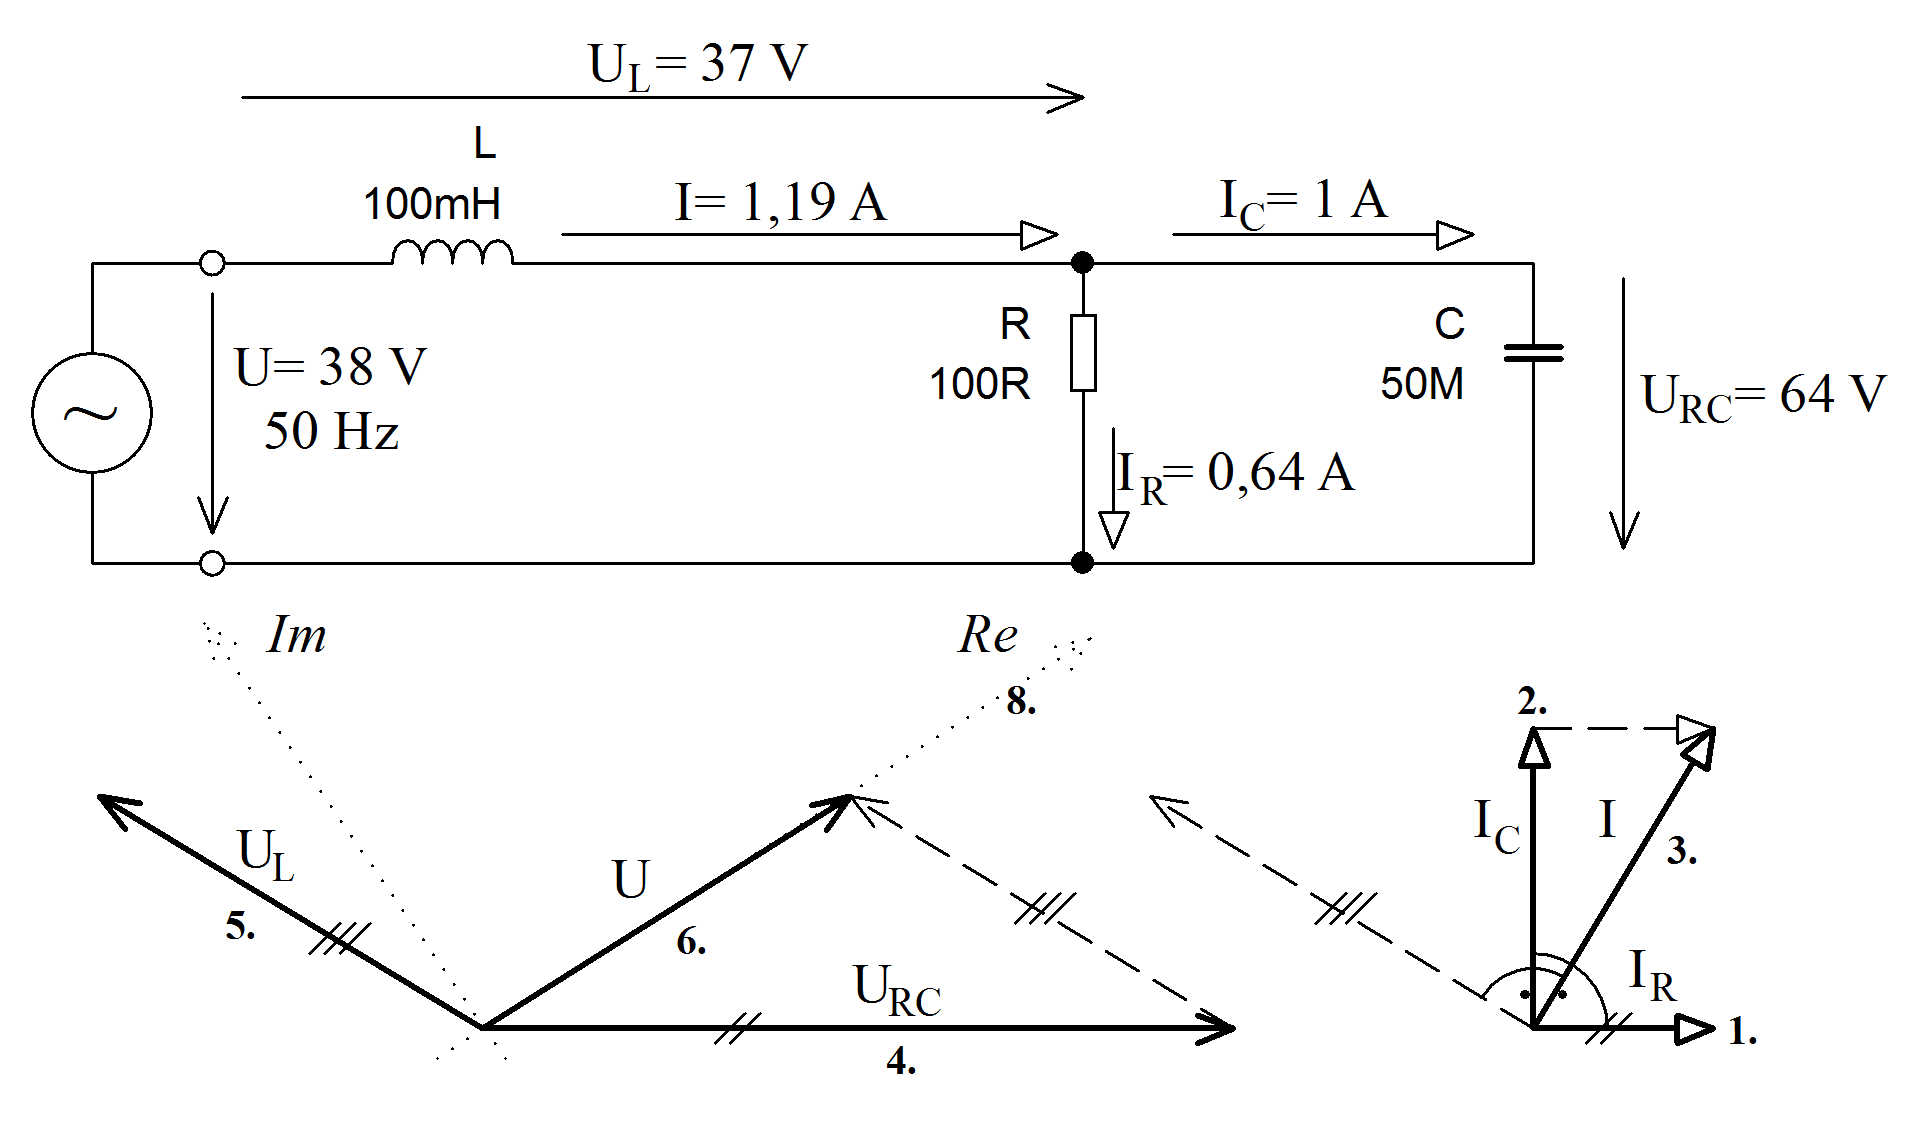
\includegraphics[width=0.80\columnwidth]{id_soucastky/fazDiag}
	\caption{Uk�zka kreslen� f�zorov�ho diagramu}
  \label{fig:idSouc:fazDiag}
\end{figure}

\subsubsection{\texorpdfstring{Rezonance}{Rezonance}}
P�i s�riov�m resp. paraleln�m spojen� induktoru a kapacitoru m��e doj�t k jevu, kdy se o f�zory nap�t� resp. proudu vz�jemn� kompenzuj� (ode�tou) a obvod dos�hne nejni��� resp. nejvy��� mo�n� impedance. K dan�mu jevu dojde kdy� se absolutn� hodnoty kapacitn� a induktivn� reaktance rovnaj�. Z t�to podm�nky lze odvodit tzv. Thompson�v vztah pro rezonanci:

\begin{equation}
\omega _{REZ}L = \frac{1}{\omega _{REZ} C} \Longrightarrow \omega _{REZ} = 2\cdot \pi \cdot f_{REZ} = \frac{1}{\sqrt{LC}}
\label{eq:idSouc:thompson}
\end{equation}

%---------------------------------------------
\newpage
\subsection{\texorpdfstring{M��en� impedance a frekven�n� vlastnosti obvodov�ch prvk�}{Mereni impedance obvodovych prvku}}

\subsubsection{\texorpdfstring{�kol m��en�}{Ukol mereni}}
\begin{enumerate}
 \item [a)] Pomoc� funk�n�ho gener�toru a osciloskopu identifikujte typ obvodov�ho prvku, kter� je p�ipojen uvnit� m��en�ho p��pravku mezi svorkami: 2-1, 3-1, 4-1;
 \item [b)] Ur�ete hodnoty hlavn�ch parametr� jednotliv�ch prvk� (R, L, C);
 \item [c)] Zm��te z�vislosti impedanc� dan�ch prvk� na frekvenci v rozsahu 200~Hz a� 2~kHz.
\end{enumerate}

\subsubsection{\texorpdfstring{Sch�ma zapojen�}{Schema zapojeni}}

\begin{figure}[h]
  \centering
  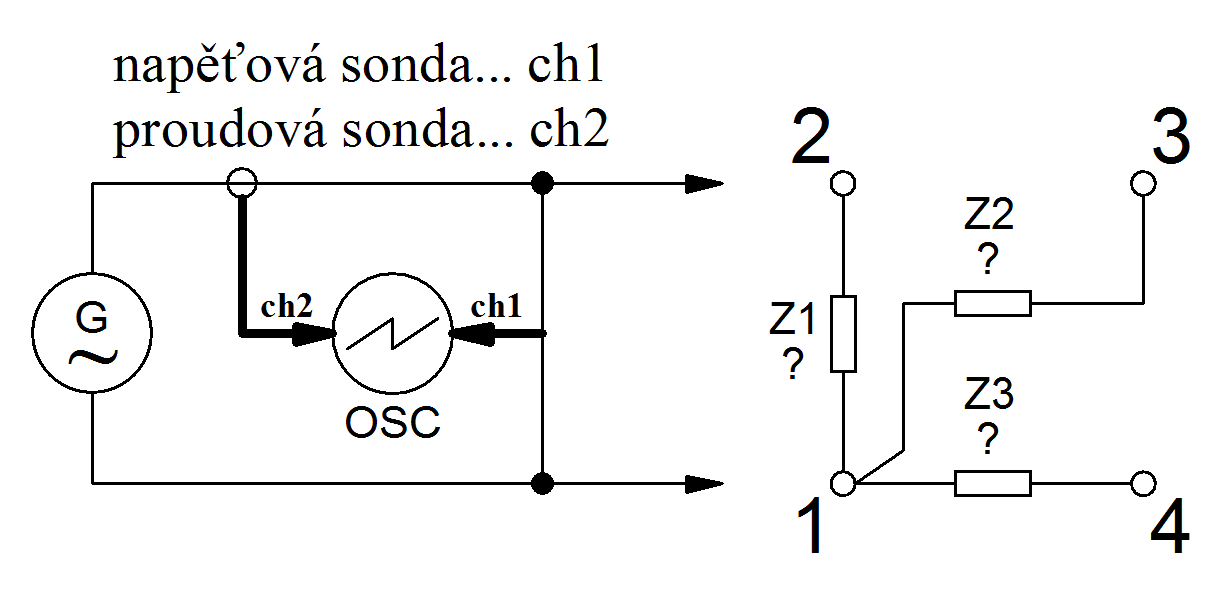
\includegraphics[width=0.60\columnwidth]{id_soucastky/blckBox}
  \label{fig:idSouc:blckBox}
\end{figure}

\subsubsection{\texorpdfstring{Postup m��en�}{Postup mereni}}

\begin{description}
 \item [ad a)] Dle sch�matu zapojen� p�ipojte osciloskop a funk�n� gener�tor k m��en�mu p��pravku. Na funk�n�m gener�toru nastavte sinusov� pr�b�h o amplitud� 5~V a frekvenci 500~Hz. Z pr�b�h� na osciloskop u vysledujte, zda existuje kladn� nebo z�porn� f�zov� posun mezi nap�t�m a proudem. D�le zm��te frekvenci na 200~Hz a 1~kHz a sledujte, zda a jak se m�n� amplituda m��en�ho proudu. Uveden� zopakujte pro v�echny impedance.
 \item [ad b)] Z hodnot z p�ede�l�ho m��en� nebo dal��m m��en�m stanovte z Ohmova z�kona hodnotu impedance. Podle typu obvodov�ho prvku dopo��tejte hlavn� parametr:
 
 \item [ad c)] Zapojen� z�st�v� nezm�n�no. Zm��te z�vislost amplitudy (p��p. efektivn� hodnoty) proudu dan�m prvkem a nap�t� (nem�n� se) na frekvenci v rozsahu 200~Hz a� 2~kHz. Frekvenci nastavujte pomoc� funk�n�ho gener�toru. Ze zm��en�ch obvodov�ch veli�in ur�ete podle Ohmova z�kona impedance a vyneste je do spole�n�ho grafu v z�vislosti na frekvenci.
\end{description}

\subsubsection{\texorpdfstring{M��en� vzorky}{Merene vzorky}}
\begin{tabular}{ll}
 1.& Black box - p��pravek RLC s nepopsan�mi vstupy \\
\end{tabular}

%---------------------------------------------
\newpage
\subsection{\texorpdfstring{M��en� RLC - f�zorov� diagramy}{Mereni RLC - fazorove diagramy}}

\subsubsection{\texorpdfstring{�kol m��en�}{Ukol mereni}}
Na osciloskopu zobrazte pr�b�hy nap�t� a proudu u jednotliv�ch spojen� pasivn�ch obvodov�ch prvk�:

\begin{tabular}{ll}
 obv. 1.& rezistor samostatn�,  \\
 obv. 2.& kapacitor samostatn�,  \\
 obv. 3.& induktor samostatn�,  \\ 
 obv. 4.& s�riov� spojen� kapacitoru a rezistoru,  \\
 obv. 5.& s�riov� spojen� induktoru a rezistoru,  \\
 obv. 6.& paraleln� spojen� rezistoru a kapacitoru,  \\ 
 obv. 7.& s�riov� spojen� induktoru a kapacitoru,  \\ 
 obv. 8.& paraleln� spojen� induktoru a kapacitoru.  \\ 
\end{tabular}

Nam��en� obvodov� veli�iny zakreslete do vektorov�ch diagram�. U obvod� obsahuj�c�ch spojen� induktoru a kapacitoru vypo�t�te rezonan�n� frekvenci. Zjist�te, zda jsou tyto obvody v rezonanci. Hodnoty hlavn�ho parametru jednotliv�ch obvodov�ch prvk� ur�ete ohmovou metodou tak, jak byly ur�ov�ny v p�edch�zej�c�m �kolu m��en� v bod� b). Z�skan� v�sledky porovnejte s m��en�m na RLC m�stku.

\subsubsection{\texorpdfstring{Sch�ma zapojen�}{Schema zapojeni}}

\begin{figure}[h]
  \centering
  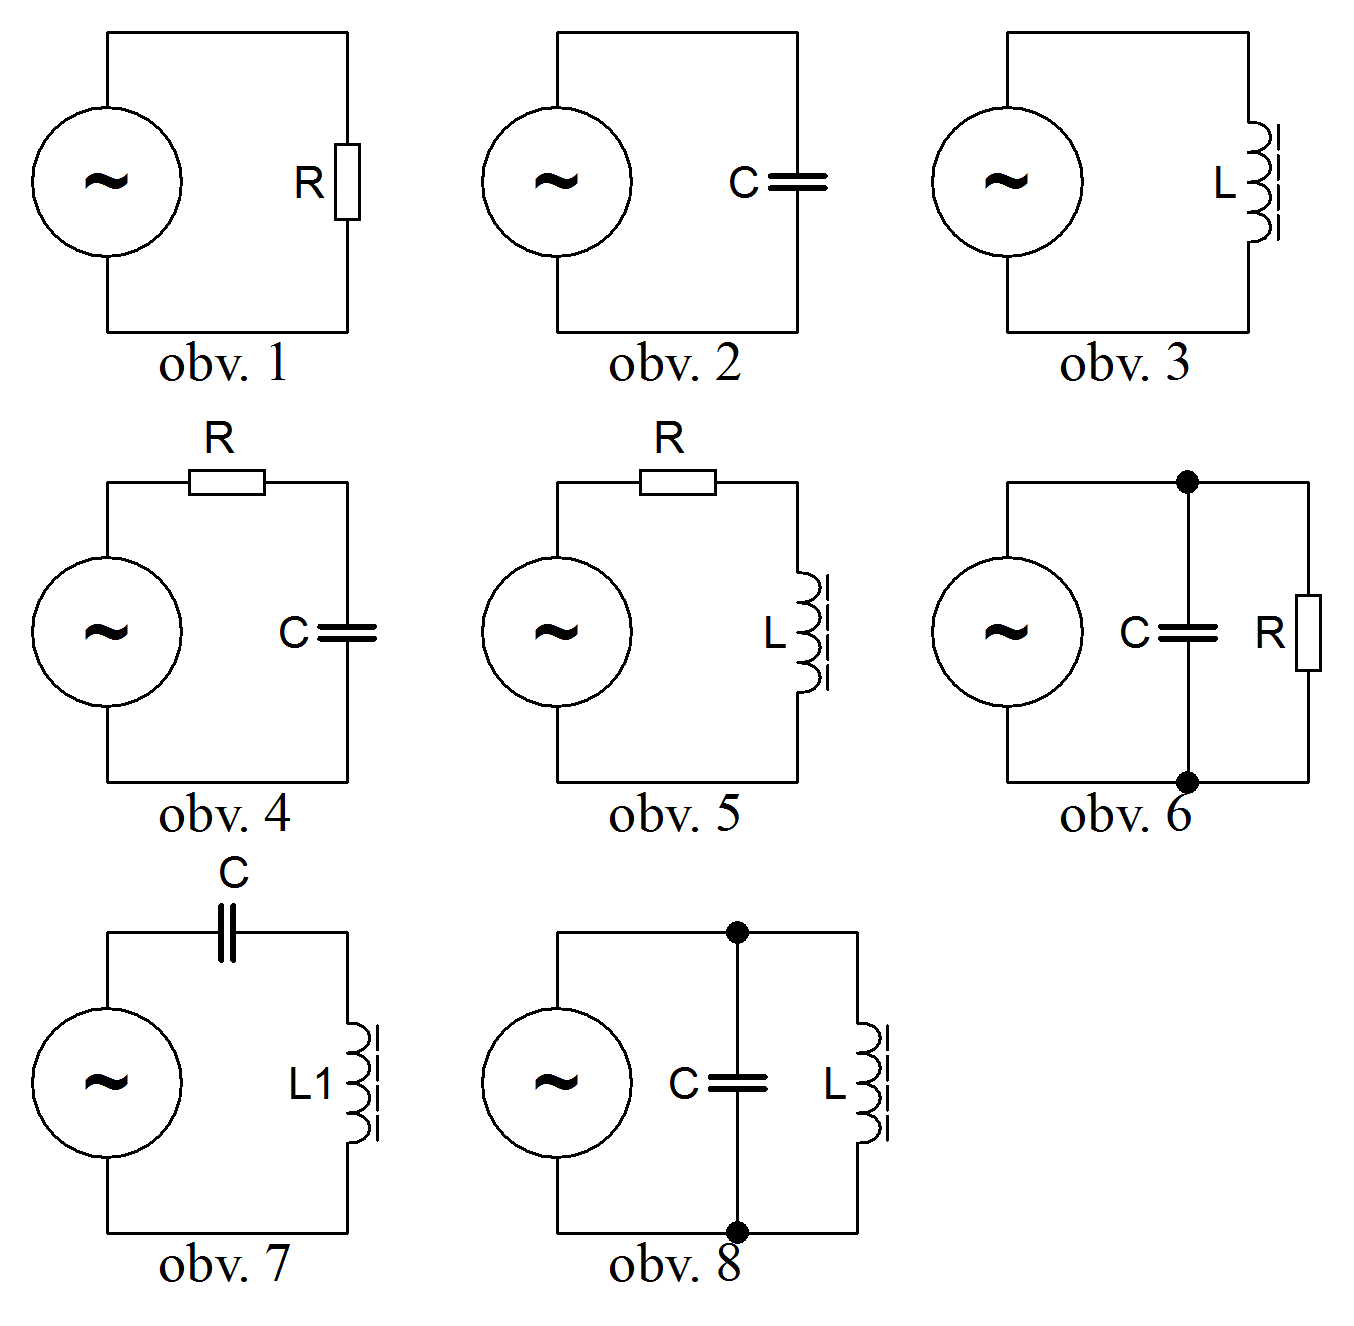
\includegraphics[width=0.65\columnwidth]{id_soucastky/idSouc}
  \label{fig:idSouc:idSouc}
\end{figure}

\subsubsection{\texorpdfstring{Postup m��en�}{Postup mereni}}
Jednotliv� obvody zapojujte dle sch�mat zapojen�. Pro nap�jen� obvod� vyu��vejte \textbf{v�hradn�} p�ipraven�ho zdroje vyhlazen� sinusovky o frekvenci 50~Hz. Tento zdroj m� m�kkou v�stupn� charakteristiku (nenulov� vnit�n� odpor), jeliko� n�kter� obvodov� spojen� vytv��ej� velmi malou v�slednou impedanci. Nap�jen� jin�m zdrojem (s tvrdou charakteristikou) m��e zp�sobit jeho zni�en� nebo destrukci sou��stek.

Ka�d� zde m��en� obvod m� jednu spole�nou obvodovou veli�inu. V p��pad� s�riov�ch spojen� te�e skrz v�echny sou��stky stejn� proud, u paraleln�ch spojen� je na v�ech sou��stk�ch shodn� nap�t�. Tuto spole�nou veli�inu v�dy uva�ujte jako referen�n� (f�zov� �hel je $\varphi = 0^\circ$, tj. f�zor ukazuje ve sm�ru re�ln� osy). V��i referen�n� hodnot� obvodov� veli�iny m��te f�zov� posuny ostatn�ch veli�in. Pro takto jednoduch� obvody t�mto zp�sobem v�dy z�sk�me ve f�zorov�m diagramu veli�iny na odporu ve sm�ru re�ln� osy a na reaktanc�ch ve sm�ru imagin�rn� osy.

\textbf{POZOR:} P�i zobrazov�n� pr�b�h� by m�ly b�t sondy osciloskopu umis�ov�ny ve stejn�m smyslu, v jak�m uva�ujeme tok proudu a j�m vyvolan� �bytky nap�t� (a� m��en� respektuje Kirchhoffovy z�kony). P�i prohazov�n� konc� sond m��e doj�t k ne��douc�mu posunu pr�b�hu o $180^\circ$.

F�zorov� diagramy vyn�ejte v amplitud�ch, tj. z osciloskopu ode��tejte v�dy amplitudy pr�b�h�. Je vhodn� zaznamenat si v�echny nam��en� hodnoty (v�dy amplituda + f�ze) do tabulky a pak teprve vyn�st jednotliv� f�zorov� diagramy.

\subsubsection{\texorpdfstring{M��en� vzorky}{Merene vzorky}}
\begin{tabular}{ll}
 1.& Dr�tov� rezistor \\
 2.& Foliov� kondenz�tor \\
 3.& C�vka na j�d�e z magnetick�ch plech� \\
\end{tabular}
%\section{\texorpdfstring{Polovodi�ov� sou��stky}{Polovodicove soucastky}}

\subsection{\texorpdfstring{�vod}{Uvod}}

Polovodi�ov� sou��stky jsou ned�lnou sou��st� modern�ch elektronick�ch za��zen�. Nej\-po\-u\-��\-va\-n�j\-��\-mi prvky jsou p�edev��m diody a tranzistory. Oba prvky maj� neline�rn� charakteristiky (vztah mezi proudy a nap�t�mi) a ke spr�vn�mu n�vrhu obvodu je nutn� tyto charakteristiky zn�t nebo zm��it.

\subsubsection{\texorpdfstring{Diody}{Diody}}

Diody jsou sou��stky s jedn�m p�echodem PN nebo s p�echodem kov polovodi� (Schottkyho dioda). Tyto prvky maj� r�zn� uplatn�n� z�visej�c� na parametrech VA charakteristiky. Ta vypad� tvarov� t�m�� v�dy stejn�, viz obr�zek~\ref{fig:polovodice:charDioda}. Hlavn� odli�nosti se t�kaj� hodnot prahov�ho nap�t� $U_{FM}$ v propustn�m sm�ru a pr�razn�ho nap�t� $U_{BR}$ v z�v�rn�m sm�ru. Usm�r�ovac� diody se vyzna�uj� mal�m nap�t�m v propustn�m sm�ru (0,3~V Schottkyho dioda, 0,6~V k�em�kov� dioda s p�echodem PN), ale velk�m pr�razn�m nap�t�m (��dov� stovky volt�). Naproti tomu Zenerovy diody maj� pr�razn� nap�t� n�zk�. To b�v� v z�vislosti na dotaci od zhruba 4~V do v�ce ne� 100~V. R�zn� hodnota pr�razn�ch (Zenerov�ch) nap�t� $U_Z$ t�chto diod se v obvodech vyu��v� jako nap�ov� reference. V�imn�te si v charakteristik�ch, �e po p�ekro�en� ur�it� hodnoty proudu se nap�t� na diod� m�n� jen m�lo. Nejv�t�� nap�t� v propustn�m sm�ru maj� zpravidla LED (Light Emitting Diode). Jeliko� nap�t� v propustn�m sm�ru i barva sv�teln�ho z��en� jsou z�visl� na ���ce zak�zan�ho p�su polovodi�e, li�� se nap�t� LED nav�c podle barvy vyza�ovan�ho sv�tla.

\begin{figure}[h]
  \centering
  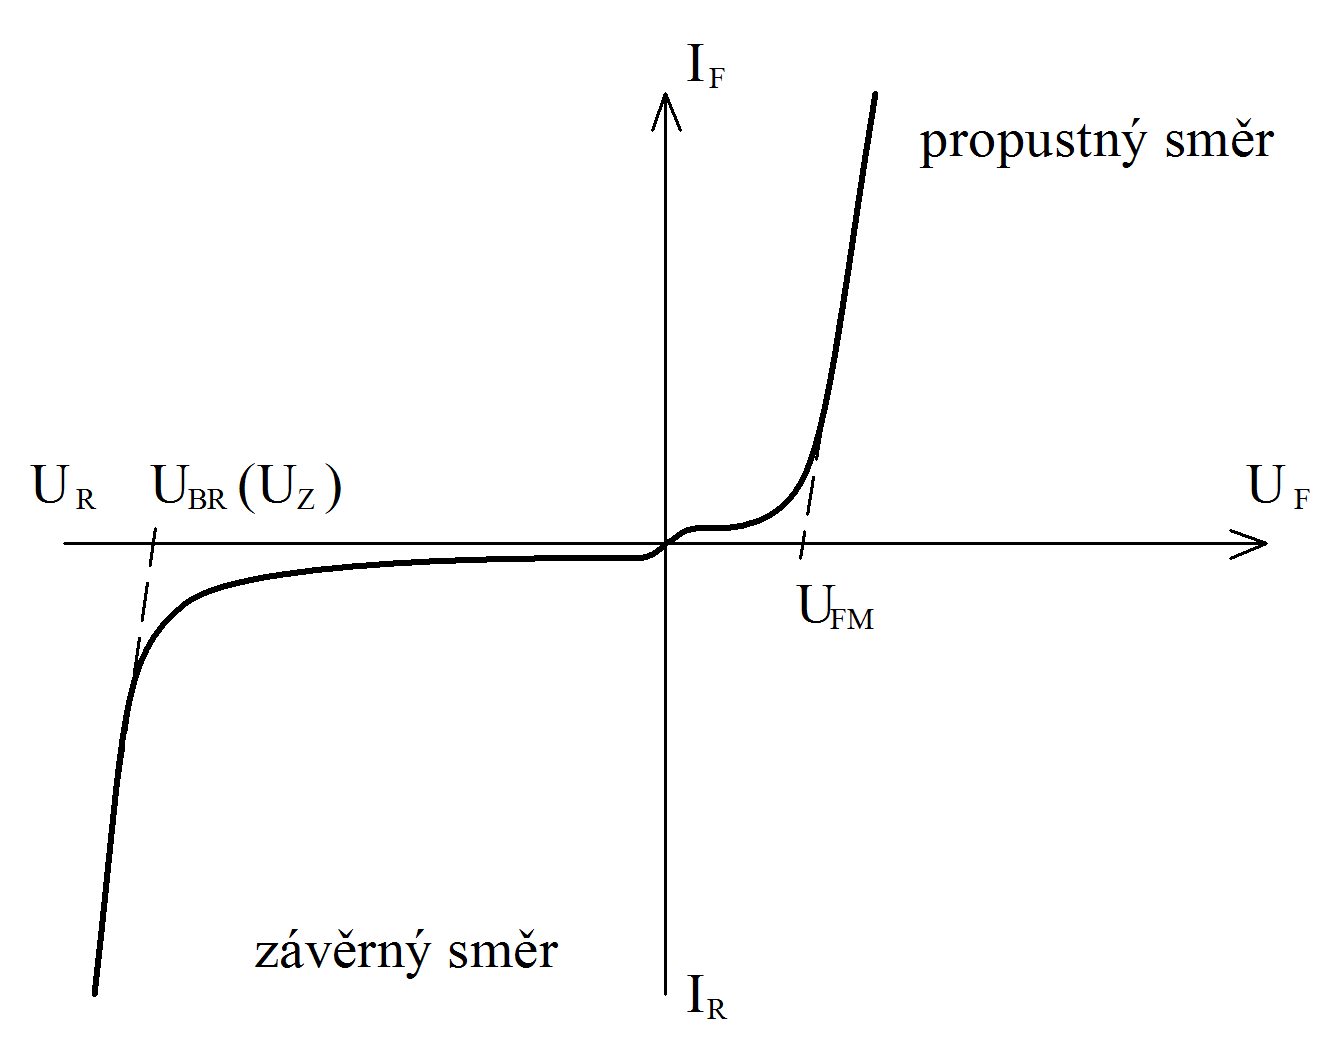
\includegraphics[width=0.5\columnwidth]{polovodice/charDioda}
	\caption{VA charakteristika diody}
  \label{fig:polovodice:charDioda}
\end{figure}

\subsubsection{\texorpdfstring{Bipolarni tranzistor}{Bipolarni tranzistor}}

Bipol�rn� tranzistor je polovodi� se dv�ma p�echody PN, kter� je p�ev�n� pou��v�n pro zesilov�n� nebo pro sp�nac� ��ely. Podle struktury rozli�ujeme typ NPN a PNP. Jedn� se o t�� v�vodovou sou��stku s elektrodami: kolektor (C), emitor (E) a b�ze (B). Velikost prot�kaj�c�ho proudu mezi kolektorem a emitorem je z�visl� na velikosti proudu prot�kaj�c�ho mezi b�z� a emitorem. Obvodov� lze tedy na tranzistor pohl�et jako na zdroj proudu �iditeln� proudem.

Tranzistor je pokl�d�n za dvojbran, p�i�em� v tomto m��en� je emitorov� v�vod spole�n� ob�ma bran�m. Vlastnosti tohoto zapojen� lze popsat pomoc� r�zn�ch typ� charakteristik. V kataloz�ch se p�ev�n� uv�d�j� hybridn� h parametry. Tranzistorov� dvojbran je tedy pops�n n�sleduj�c� soustavou rovnic:

\begin{equation}
U_{BE} = h_{11E} \cdot I_{B} + h_{12E} \cdot U_{CE}
\label{eq:polovodice:hparUbe}
\end{equation}

\begin{equation}
I_{C} = h_{21E} \cdot I_{B} + h_{22E} \cdot U_{CE}
\label{eq:polovodice:hparIc}
\end{equation}

\noindent
Jednotliv� parametry, jak u� jejich jednotky napov�daj�, maj� r�zn� v�znamy:
\begin{description}
\item{$h_{11E}$} je vstupn� impedance tranzistoru ($\Omega$),
\item{$h_{12E}$} je zp�tn� nap�ov� p�enos (-),
\item{$h_{21E}$} je proudov� zesilovac� �initel (-),
\item{$h_{22E}$} je v�stupn� admitance tranzistoru (S).
\end{description}

\noindent
$h$ parametry lze pokl�dat za konstantn� pouze pro ur�it� okol� pracovn�ho bodu. Pro r�zn� pracovn� body se jejich hodnoty obvykle li��. Proto se vlastnosti tranzistoru popisuj� mimojin� graficky vynesen�m jednotliv�ch charakteristik ze zm��en�ch dat.

\begin{figure}[h]
  \centering
  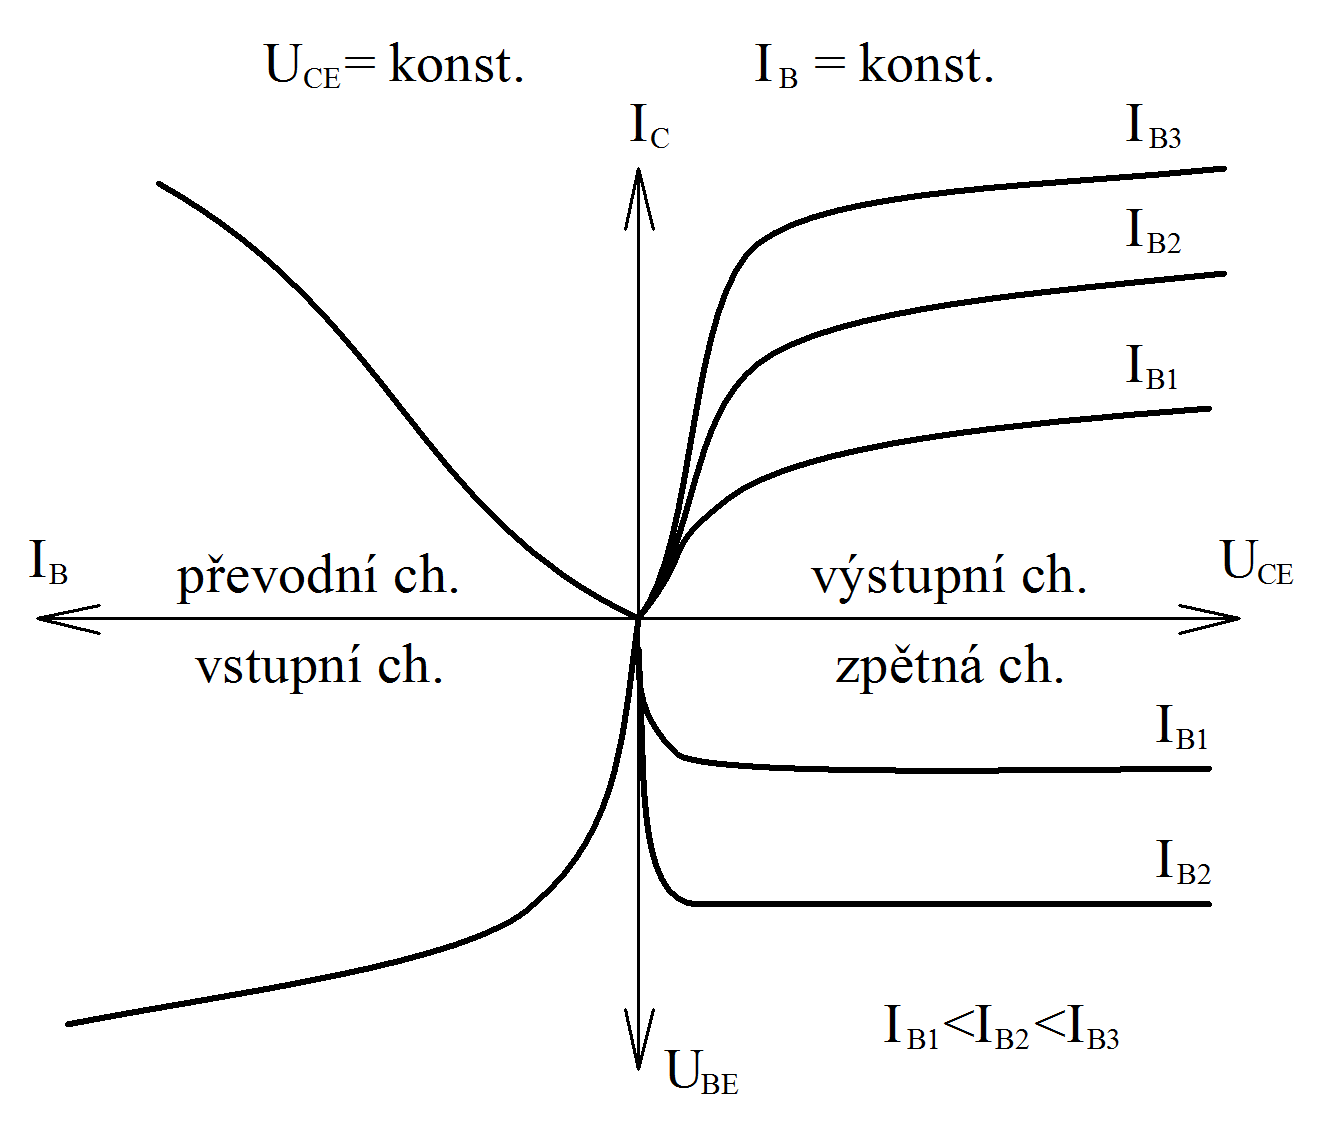
\includegraphics[width=0.5\columnwidth]{polovodice/charTransistor}
	\caption{VA charakteristika tranzistoru}
  \label{fig:polovodice:charTransistor}
\end{figure}

\subsubsection{\texorpdfstring{M��en� VA charakteristiky pulzn� metodou}{Pulzni metoda}}

VA charakteristika polovodiv�ho prvku v�dy z�vis� na teplot�. P�i statick�m m��en� stejnosm�rn�m proudem doch�z� vlivem ztr�t k oh��v�n� m��en�ho prvku. P�i pomal�m m��en� jsou tak jednotliv� body charakteristiky zm��eny p�i r�zn�ch teplot�ch. Do VA charakteristiky m��eme takto zavl�ci i ur�itou hysterezi, pokud budeme m��it z nulov�ho proudu do maxima a n�sledn� zp�t. Pracovn� bod oh��t�ho prvku toti� pob�� po jin� k�ivce.

Oh��v�n� prvku se vyhneme nap�jen�m prvku co nejni��� efektivn� hodnotou m���c�ho proudu. Sn�en� efektivn� hodnoty proudu, ani� bychom museli m�nit m��en� rozsah proudu, dos�hneme nap�jen�m pomoc� pulz�. Cel� m��en� tak prob�hne v r�mci jednoho kr�tk�ho pulzu a nedojde k v�razn�mu oh��t� sou��stky. 

%---------------------------------------------
\newpage
\subsection{\texorpdfstring{M��en� VA charakteristik r�zn�ch typ� diod}{Mereni VA charakteristik diod}}

\subsubsection{\texorpdfstring{�kol m��en�}{Ukol mereni}}

Zm��te VA charakteristiky I=f(U) v propustn�m sm�ru p�edlo�en�ch polovodi�ov�ch diod. Nam��en� hodnoty vyneste do grafu a vz�jemn� je porovnejte. Vyberte si jednu diodu, jej� charakteristiku zm���te statickou metodou. Charakteristiky ostatn�ch diod m��te pulzn� gener�torem a osciloskopem. U Zenerovy diody nav�c zm��te a vyneste i charakteristiku v z�v�rn�m sm�ru.

\subsubsection{\texorpdfstring{Sch�ma zapojen�}{Schema zapojeni}}

\begin{figure}[h]
  \centering
  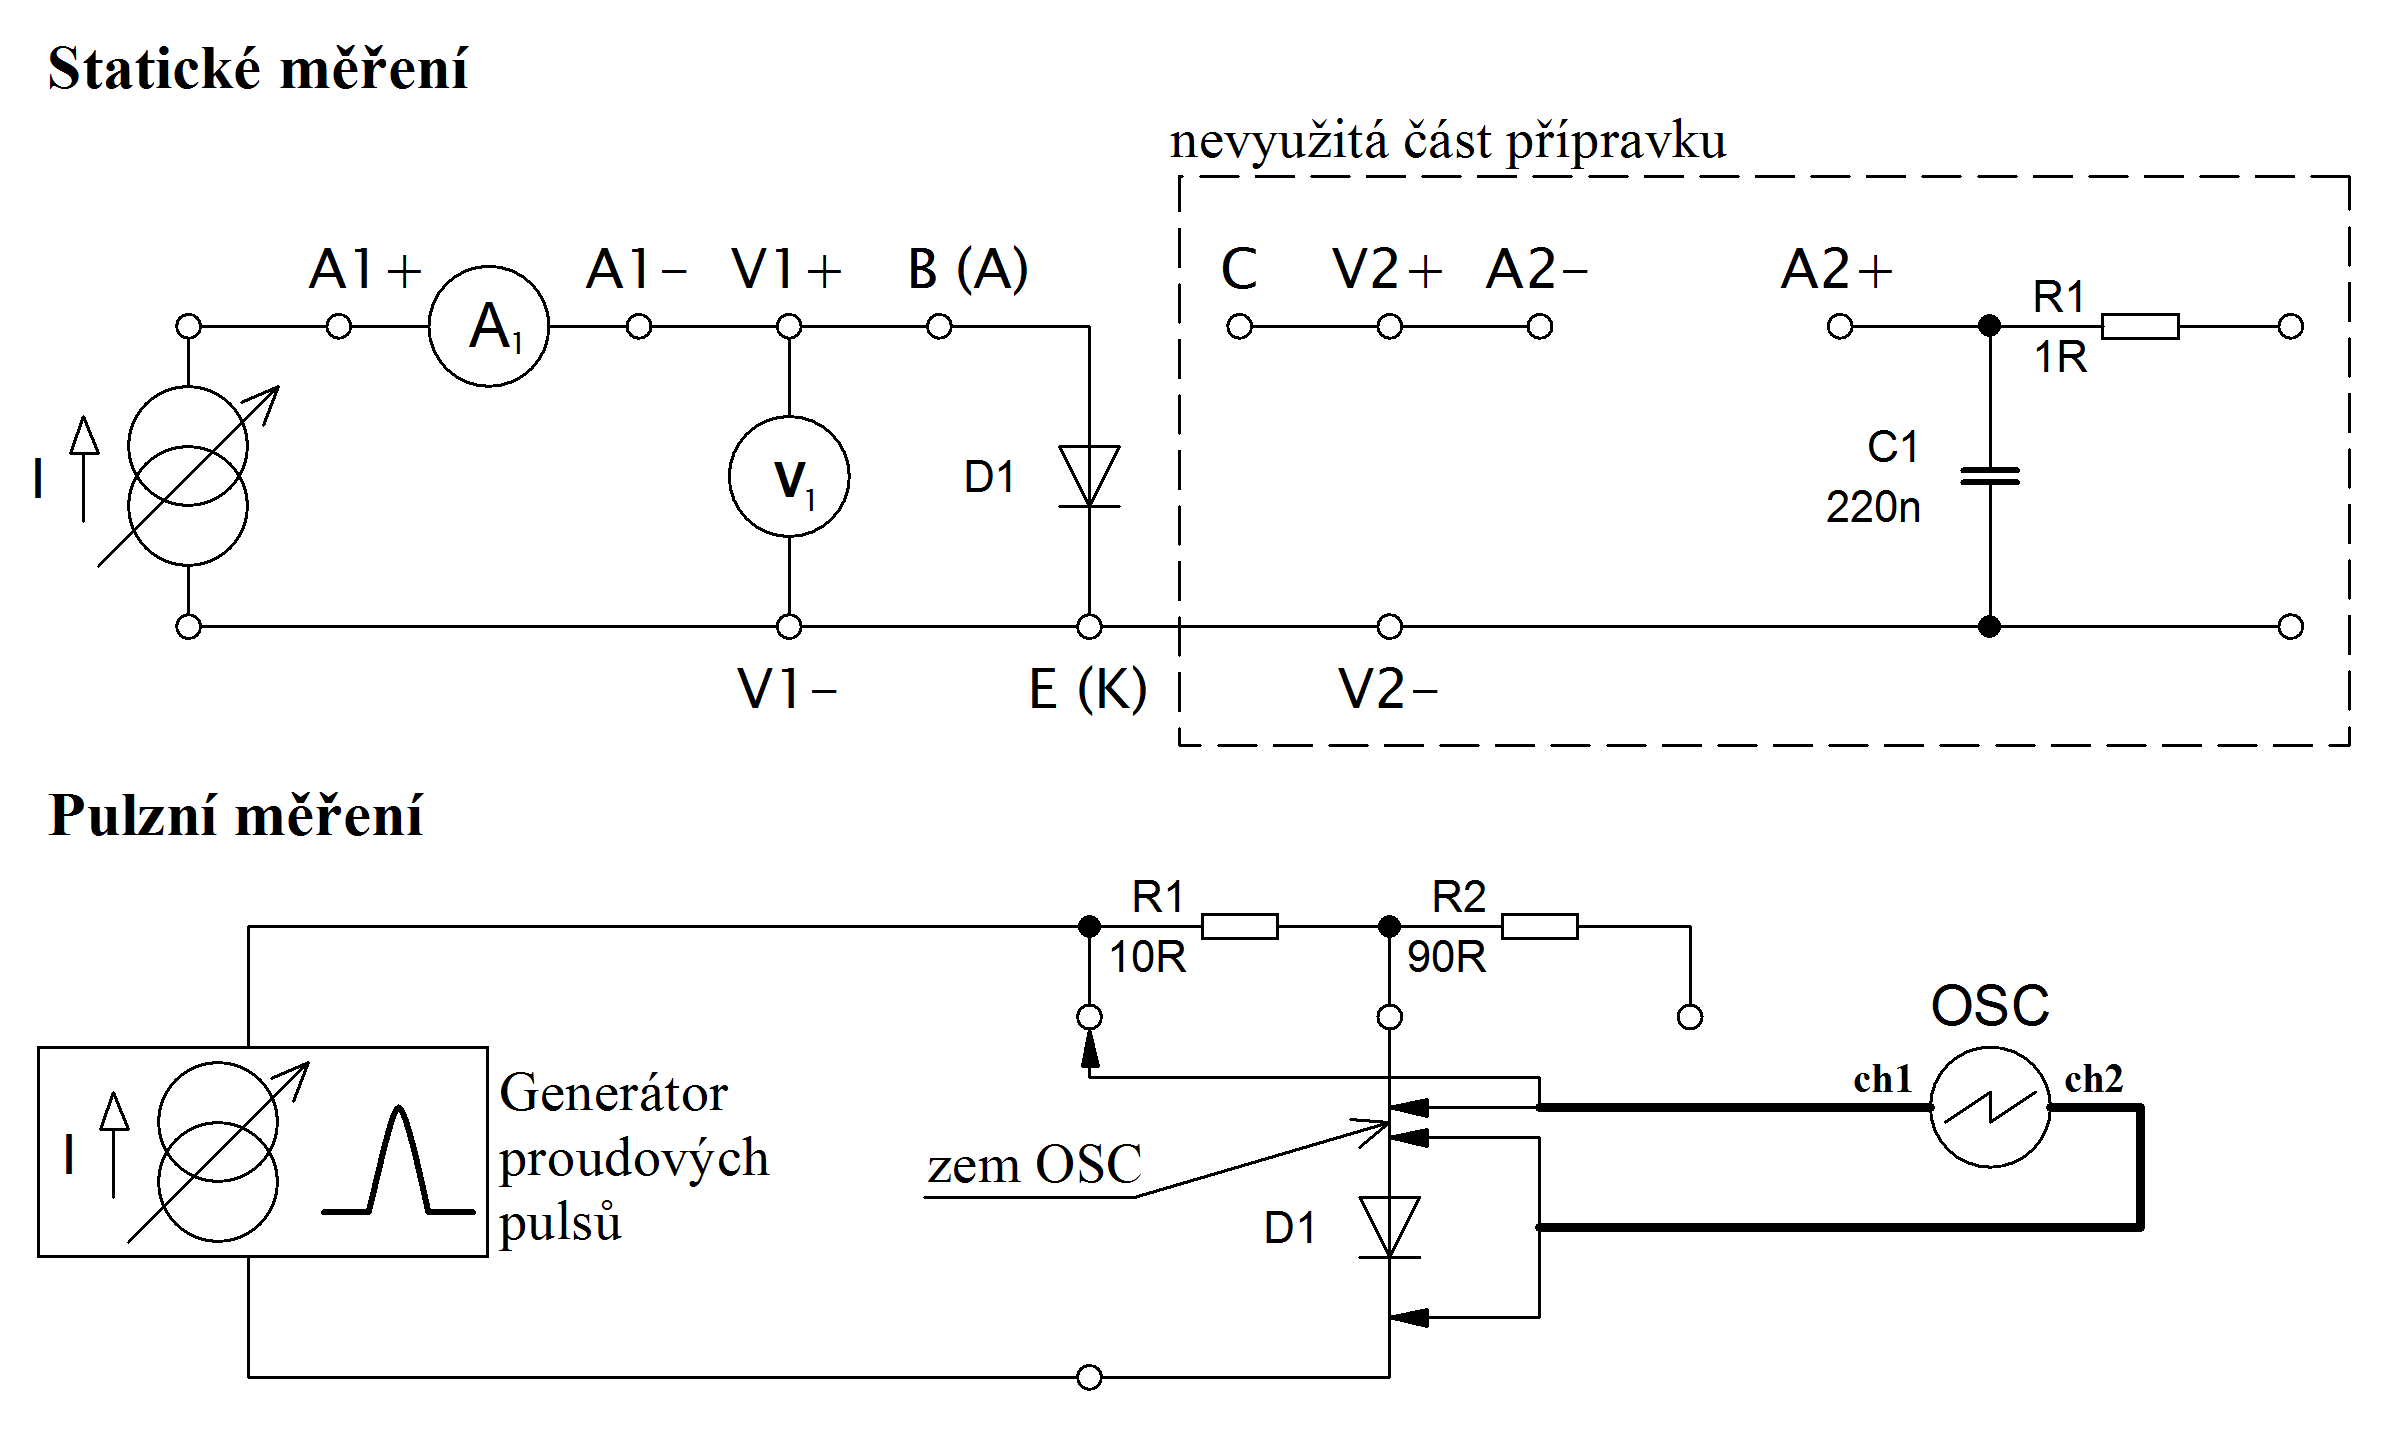
\includegraphics[width=0.90\columnwidth]{polovodice/polDioda}
  \label{fig:polovodice:polDioda}
\end{figure}

\subsubsection{\texorpdfstring{Postup m��en�}{Postup mereni}}
P�i statick�m m��en� pou�ijte p��pravek pro m��en� VA charakteristik tranzistoru a obvod zapojte dle p��slu�n�ho sch�ma zapojen�. Propustn� sm�r diody bude m��en, pokud bude anoda p�ipojena na svorku B (b�ze) a katoda na svorku E (emitor). Pro vzorky 1,2,3 a 5 m��te v rozsahu proud� 0-200~mA. U vzorku 4 m��te jen do maxima proudu 20~mA. Nastaven� proud ode��tejte z amp�rmetru A$_1$ a vznikl� �bytek nap�t� z voltmetru V$_1$. Charakteristika v�ech diod je prudce neline�rn�. Pro snadn� vyn�en� do grafu je t�eba podrobn� prom��it oblast kolene vyn�en� k�ivky. Proto danou oblast, kde se nap�t� s proudem prudce m�n�, m��te s velmi mal�m krokem proudu.

U pulsn�ho m��en� p�ipojujte jednotliv� diody na m���c� svorky dle sch�ma zapojen� a zobrazujte jejich VA charakteristiky v XY re�imu na osciloskopu. Data sejm�te ve form�tu CSV a ulo�te na vhodn� medium (flash disk). V tomto p��pad� grafy p�i zpracov�n� vyneste za pomoci odpov�daj�c�ho softwaru - EXCEL, MATLAB apod. Nap�t� bude v datech zobrazeno p��mo, av�ak proud je sn�m�n jako �bytek nap�t� na 10~$\Omega$ odporu. Proto prove�te p��slu�n� p�epo�et! Pokud m�te danou mo�nost, otestujte jak se zm�n� VA charakteristika vlivem zm�ny teploty.

\subsubsection{\texorpdfstring{M��en� vzorky}{Merene vzorky}}
\begin{tabular}{ll}
 1.& Shottkyho dioda typ 1N5819, parametry $I_{max}$= 1 A, $U_{max}$= 40 V. \\
 2.& K�em�kova dioda univerz�ln� typ 1N4007, parametry $I_{max}$= 1 A, $U_{max}$= 1000 V. \\ 
 3.& LED 5 mm b�l� 9000 mcd, parametry $U_f$= 4 V, $I_{max}$= 100 mA. \\ 
 4.& LED 10 mm �erven�, parametry $U_f$= 1,9 V, $I_{max}$= 20 mA. \\ 
 5.& Zenerova dioada typ 1N5337, parametry $U_{z}$= 4,7 V, $I_{zmax}$= 1 A, $P_{max}$= 5 W. \\
\end{tabular}

%---------------------------------------------
%\newpage
\subsection{\texorpdfstring{M��en� stejnosm�rn�ch charakteristik tranzistoru}{Mereni stejnosmernych charakteristik tranzistoru}}

\subsubsection{\texorpdfstring{�kol m��en�}{Ukol mereni}}

\begin{enumerate}
 \item [a)] Zm��te v�stupn� charakteristiky p�edlo�en�ch tranzistor� v zapojen� se spole�n�m emitorem pro proudy b�ze $I_B$ = 1, 2, 5, 10~mA. P�i m��en� nep�es�hn�te maxim�ln� mez stejnosm�rn�ho nap�t� 20~V v kolektorov�m obvod� tranzistoru.
 \item [b)] Zm��te p�evodn� charakteristiku p�edlo�en�ch tranzistor� pro nap�t� $U_{CE}$=~10~V.
 \item [c)] Zm��te vstupn� charakteristiku p�edlo�en�ch tranzistor� pro nap�t� $U_{CE}$=~10~V.
\end{enumerate}

\subsubsection{\texorpdfstring{Sch�ma zapojen�}{Schema zapojeni}}

\begin{figure}[h]
  \centering
  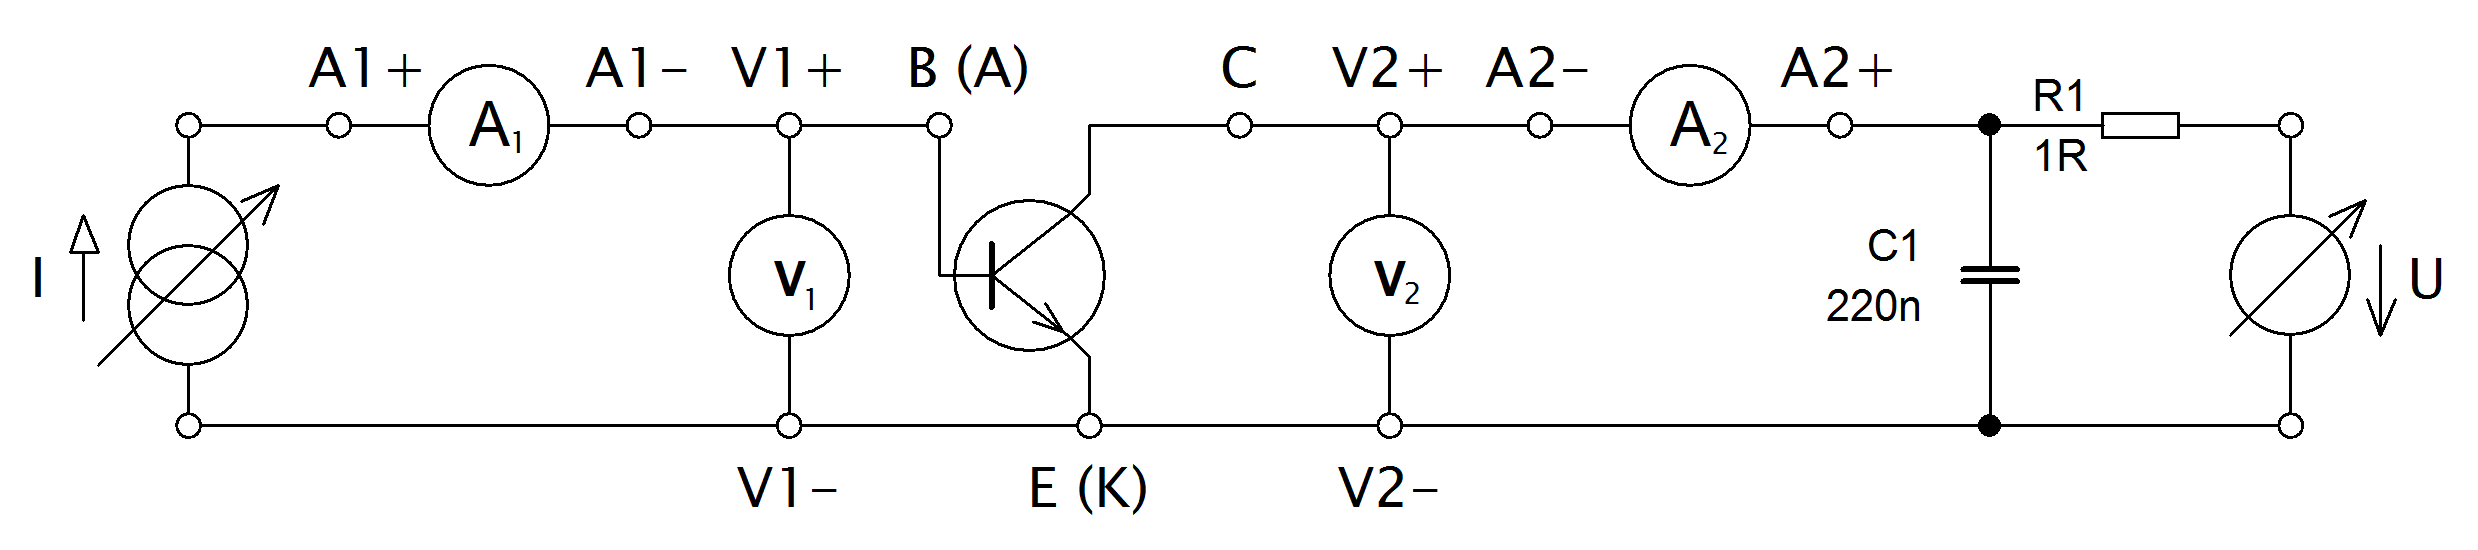
\includegraphics[width=0.90\columnwidth]{polovodice/polTransistor}
  \label{fig:polovodice:polTransistor}
\end{figure}

\subsubsection{\texorpdfstring{Postup m��en�}{Postup mereni}}

\begin{description}
 \item [ad a)] Regulovateln�m proudov�m zdrojem I (knofl�kem na p��pravku) nastavte po�adovan� proud obvodem b�ze. Pomoc� regulovateln�ho nap�ov�ho zdroje U, amp�rmetru A$_2$ a voltmetru V$_2$ nastavujte nap�t� a m��te proud obvodem kolektoru. Nap�t� nastavujte v rozsahu 0 � 10 V.
 \item [ad b)] Regulovateln�m nap�ov�m zdrojem U nastavte nap�t� $U_{CE}$=~10~V. Pomoc� regulovateln�ho proudov�ho zdroje I, amp�rmetru A$_1$ a A$_2$ nastavujte proud b�z� $I_B$ a m��te proud obvodem kolektoru $I_C$. Proud kolektorem nesm� p�es�hnout hodnotu 1,2~A.
 \item [ad c)] Regulovateln�m nap�ov�m zdrojem U nastavte nap�t� $U_{CE}$=~10~V. Pomoc� regulovateln�ho proudov�ho zdroje U, amp�rmetru A$_1$ a voltmetru V$_2$ nastavujte proud b�z� $I_B$ a m��te nap�t� mezi b�z� a emitorem. Proud kolektorem nesm� p�es�hnout hodnotu 1,2~A.
\end{description}

Nam��en� hodnoty zapisujte do tabulek a z�rove� je vyn�ejte na milimetrov� pap�r. Tabulky i vynesen� charakteristiky si n�sledn� �lenov� skupiny okop�ruj� do vlastn�ch se�it� (existuje 1 origin�l tabulky a 1 origin�l charakteristiky!!).

\subsubsection{\texorpdfstring{M��en� vzorky}{Merene vzorky}}
\begin{tabular}{ll}
 1.& BD239, tranzistor NPN, $U_{CE} =$~100~V, $I_C =$~2~A \\
 2.& BD711, tranzistor NPN, $U_{CE} =$~100~V, $I_C =$~12~A \\
\end{tabular}
%\section{\texorpdfstring{Porovn�n� VA charakteristik r�zn�ch typ� fotovoltaick�ch �l�nk�}{Porovnani VA charakteristik fotovoltaickych clanku}}

\subsection{\texorpdfstring{�vod}{Uvod}}

%---------------------------------------------
\subsection{\texorpdfstring{M��en� VA charakteristik fotovoltaick�ch �l�nk�}{Mereni VA charakteristik fotovoltaickych clanku}}

\subsubsection{\texorpdfstring{�kol m��en�}{Ukol mereni}}
Zm��te voltamp�rov� charakteristiky p�ilo�en�ch fotovoltaick�ch �l�nk� a ur�ete o jak� typ �l�nku se jedn�. U ka�d�ho typu �l�nku ur�ete:

\begin{itemize}
 \item proud nakr�tko $I_SC$,
 \item nap�t� napr�zdno $U_0C$,
 \item paraleln� odpor $R_P$ reprezentuj�c� poruchy v �l�nku,
 \item s�riov� odpor $R_S$ reprezentuj�c� elektrick� ztr�ty,
 \item bod maxim�ln�ho v�konu $MPP$ (resp. $P_{MAX}$),
 \item �initel pln�n� (fill factor) $FF$,
 \item ��innost �l�nku $\eta$.
\end{itemize}

Prove�te vz�jemn� porovn�n� jednotliv�ch parametr� mezi r�zn�mi �l�nky. Do spole�n�ho grafu vyneste charakteristiky $I= f(U)$ a $P= f(U)$ v�ech testovan�ch �l�nk� a pr�b�hy porovnejte.

\subsubsection{\texorpdfstring{Postup m��en�}{Postup mereni}}

Z�t� je realizov�na p�ep�natelnou odporovou kask�dou pro krystalick� �l�nky a posuvn�m rezistorem v p��pad� tenkovrstv�ho �l�nku. S m��en�m za��n�me v chodu napr�zdno a pot� postupn� sni�ujeme odpor a� do chodu nakr�tko. Pro chod napr�zdno rozpoj�me svorky z�t�e, pro chod nakr�tko je zkratujeme. Ode��t�me p��slu�n� hodnoty nap�t� a proudu. Cel� m��en� opakujeme pro v�echny typy �l�nk�.

\subsubsection{\texorpdfstring{M��en� vzorky}{Merene vzorky}}
\begin{tabular}{ll}
 1.& ? \\
 2.& ? \\
 3.& ? \\ 
\end{tabular}

%\section{\texorpdfstring{Vlastnosti vysokofrekven�n�ch c�vek}{Vlastnosti vysokofrekvencnich civek}}

\subsection{\texorpdfstring{�vod}{Uvod}}
Induk�nost v elektrick�m obvodu je obvykle realizov�na c�vkou, tj. uspo��d�n�m vodi�� ve tvaru z�vit�. C�vka m��e b�t navinuta z vodi�� obvykle kruhov�ho pr��ezu do v�lcov�ho nebo diskov�ho tvaru nebo nap�. vytvo�ena jako obrazec na desce plo�n�ch spoj�. Induk�nost c�vky z�vis� na po�tu z�vit�, rozm�rech vinut�, vz�jemn� poloze z�vit� a na magnetick� vodivosti prost�ed�, kter�m se uzav�raj� silo��ry magnetick�ho toku c�vky (vzduch, ferromagnetick� materi�l). P�i pou�it� c�vky v obvodech s vysok�mi frekvencemi nap�t� se v�razn� uplatn� tak� odpor a kapacity vinut�, skinefekt a vf. vlastnosti magnetick�ch materi�l�.

\subsubsection{\texorpdfstring{�initel jakosti - p�ev��en�}{Cinitel jakosti}}

Narozd�l od kondenz�tor� nelze u c�vek zanedbat parazitn� s�riov� odpor. Jen ve velmi ojedin�l�ch p��padech nen� t�eba p�i konstrukci obvodu hodnotu tohoto odporu uva�ovat, nebo� je hlavn� p���inou vzniku ztr�t a z toho plynouc�ho oh�evu c�vky (Jouleovy ztr�ty ve vinut�, ztr�ty v mag. obvodu atd.). �initel jakosti je definov�n jen v rezonan�n�ch obvodech. Zde ud�v� pom�r akumulovan� energie ku ztracen� energii.

P�i s�riov�m spojen� kondenz�toru a c�vky vznikne rezonan�n� obvod, jeho� energie se ztr�c� p�edev��m na parazitn�m odporu c�vky. Rezonan�n� $LC$ obvod tak p�ech�z� na rezonan�n� $RLC$ obvod. �bytek nap�t� na odporu je �m�rn� ztr�t�m v obvodu a nap�t� na induk�nosti (resp. kapacit�) je �m�rn� jalov�mu v�konu, tud� jde o energii akumulovanou v rezonan�n�m obvodu. Anal�zou tohoto faktu z�sk�me pro �initel jakosti vztah:

\begin{equation}
Q= \frac{\omega L}{R}
\label{eq:vfCivky:Q}
\end{equation}

Z�ejm� m��eme �initel jakosti uva�ovat jako p�evr�cenou hodnotu ztr�tov�ho �initele nebo jako pom�r imagin�rn� a re�ln� ��sti impedance c�vky. Jeliko� je odpor c�vky relativn� mal�, dosahuje �initel jakosti na frekvenc�ch ��dov� kHz hodnot ��dov� des�tek a� stovek.

\subsubsection{\texorpdfstring{Nap�t� na prvc�ch v rezonanci}{Napeti na prvcich v rezonanci}}

B�hem rezonance s�riov�ho $RLC$ obvodu doch�z� ke zv��en� amplitudy nap�t� na c�vce a kondenz�toru. Anal�zou vztah� pro impedanci a nap�t� na jednotliv�ch prvc�ch lze odvodit p�vod tohoto jevu. Zde celou v�c zjednodu��me �vahou. P�i rezonanci plat�, �e induktivn� reaktance c�vky je a� na znam�nko rovna kapacitn� reaktanci kondenz�toru. Jejich sou�et je nulov� a impedance obvodu m� pouze re�lnou ��st danou hodnotou odporu. Pro f�zor proudu tak z�sk�v�me vztah:

\begin{equation}
\widehat{I}= \frac{\widehat{U}}{\widehat{Z}}= \frac{\widehat{U}}{\widehat{R}}
\label{eq:vfCivky:Proud}
\end{equation}

Reaktance c�vky a kondenz�toru je st�le v obvodu p��tomna a proch�zej�c� proud vyvol� na obou prvc�ch nap�t�, kter� budou vz�jemn� v protif�zi (v��i sob� posunuta o 180$^\circ$):

\begin{equation}
\widehat{U}_L= \widehat{I}\cdot jX_L= \widehat{U} \cdot \frac{j\omega L}{R} = \widehat{U} \cdot jQ
\label{eq:vfCivky:napetiNaL}
\end{equation}

\begin{equation}
\widehat{U}_C= \widehat{I}\cdot (-jX_C)= \widehat{U} \cdot \frac{-j}{\omega CR} = \widehat{U} \cdot (-jQ)
\label{eq:vfCivky:napetiNaC}
\end{equation}

Z rovnic vypl�v� (\ref{eq:vfCivky:napetiNaL}) a (\ref{eq:vfCivky:napetiNaC}), �e v�sledn� nap�t� na obou reaktanc�ch bude zes�leno velikost� �initele jakosti.

%--------------------------------------
\newpage
\subsection{\texorpdfstring{M��en� frekven�n� z�vislosti �initele p�ev��en� Q}{Mereni frekvencni zavislosti cinitele previseni Q}}

\subsubsection{\texorpdfstring{�kol m��en�}{Ukol mereni}}
Zjist�te m��en�m kmito�tov� z�vislosti �initele p�ev��en� $Q$ dan�ch vzork� c�vek vliv konstruk�n�ho proveden� (d�lky vinut�, rozm�r� a formy vodi��) na jejich kvalitu. Nam��en� hodnoty vyneste do grafu! Diskutujte vliv proveden� vinut� na vlastnosti c�vky. Ov��te vliv feritov�ho j�dra na vlastnosti c�vek.

\subsubsection{\texorpdfstring{Sch�ma zapojen�}{Schema zapojeni}}

\begin{figure}[h]
  \centering
  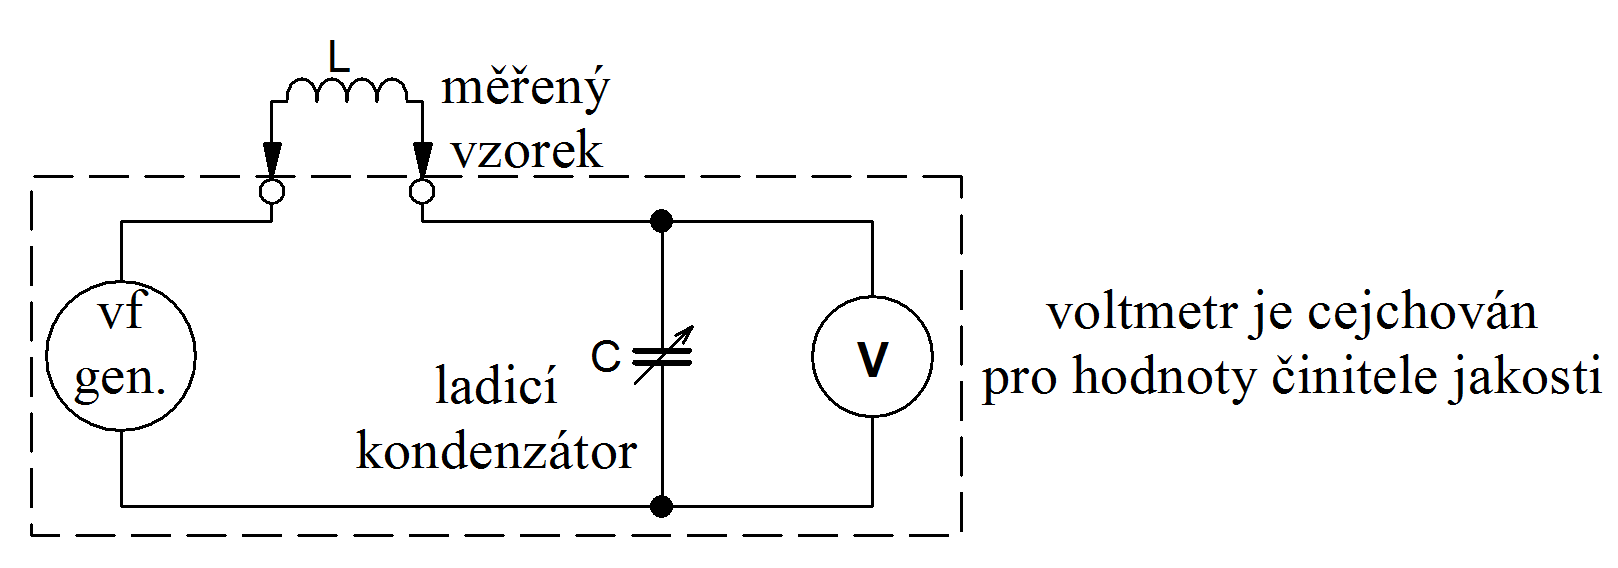
\includegraphics[width=0.7\columnwidth]{vf_civky/vfCivky}
  \label{fig:vfCivky:vfCivky}
\end{figure}

\subsubsection{\texorpdfstring{Postup m��en�}{Postup mereni}}
M��te na Q-metru v kmito�tov�m rozsahu ur�en�m nejmen�� a nejv�t�� kapacitou ladic�ho kondenz�toru p��stroje (obvod s c�vkou se lad� do rezonance).
Kmito�tov� krok volte tak, abyste u ka�d� c�vky zm��ili alespo� 5 hodnot rovnom�rn� rozlo�en�ch v kmito�tov�m intervalu. Vlo�en�m feritov�ho j�dra do c�vek 1 a� 3 (vzorky 4-6) zjist�te zm�nu jejich el. parametr�.

\subsubsection{\texorpdfstring{M��en� vzorky}{Merene vzorky}}
\begin{tabular}{ll}
 1.& c�vka D = 40 mm, l = 27 mm, 13 z�vit� vodi�em $\diameter$ 1,2 mm \\
 2.& c�vka D = 40 mm, l = 27 mm, 27 z�vit� vodi�em $\diameter$ 0,6 mm \\
 3.& c�vka D = 40 mm, l = 27 mm, 57 z�vit� vodi�em $\diameter$ 0,3 mm \\ 
 4.& c�vka D = 40 mm, l = 27 mm, 13 z�vit� vodi�em $\diameter$ 1,2 mm, feritov� j�dro z mat. N1 \\
 5.& c�vka D = 40 mm, l = 27 mm, 27 z�vit� vodi�em $\diameter$ 0,6 mm, feritov� j�dro z mat. N1 \\
 6.& c�vka D = 40 mm, l = 27 mm, 57 z�vit� vodi�em $\diameter$ 0,3 mm, feritov� j�dro z mat. N1 \\
 7.& c�vka MESC (GES Electronic), 10 $\mu$H, feritov� j�dro ty�inka \\
 8.& c�vka 09P (GM Electronic), 560 $\mu$H, feritov� j�dro c�vka \\
\end{tabular}

%--------------------------------------
\newpage
\subsection{\texorpdfstring{M��en� frekven�n� z�vislosti induk�nosti $L_S$ a �initele p�ev��en� $Q$ vzork� na feritov�ch j�drech}{Mereni frekvencni zavislosti indukcnosti Ls}}

\subsubsection{\texorpdfstring{�kol m��en�}{Ukol mereni}}
Zm��te s�riovou induk�nost LS a �initel p�ev��en� Q v z�vislosti na frekvenci. Najd�te frekvenci pro maxim�ln� hodnotu Q a frekvenci vlastn� rezonance fr. M��en� prove�te pomoc� LCR metru HP4284A.

\subsubsection{\texorpdfstring{Postup m��en�}{Postup mereni}}
M��te na Q-metru v kmito�tov�m rozsahu ur�en�m nejmen�� a nejv�t�� kapacitou ladic�ho kondenz�toru p��stroje (obvod s c�vkou se lad� do rezonance).
Kmito�tov� krok volte tak, abyste u ka�d� c�vky zm��ili alespo� 5 hodnot rovnom�rn� rozlo�en�ch v kmito�tov�m intervalu. Vlo�en�m feritov�ho j�dra do c�vek 1 a� 3 (vzorky 4-6) zjist�te zm�nu jejich el. parametr�.

\subsubsection{\texorpdfstring{M��en� vzorky}{Merene vzorky}}
\begin{tabular}{ll}
 1.& tlumivka 3,7 mH (feritov� j�dro obd�ln�kov�) \\
 2.& tlumivka 600 $\mu$H (feritov� j�dro obd�ln�kov�) \\
\end{tabular}

%--------------------------------------
\subsection{\texorpdfstring{Obr�zkov� p��loha}{Obrazkova priloha}}

\begin{figure}[h]
  \centering
  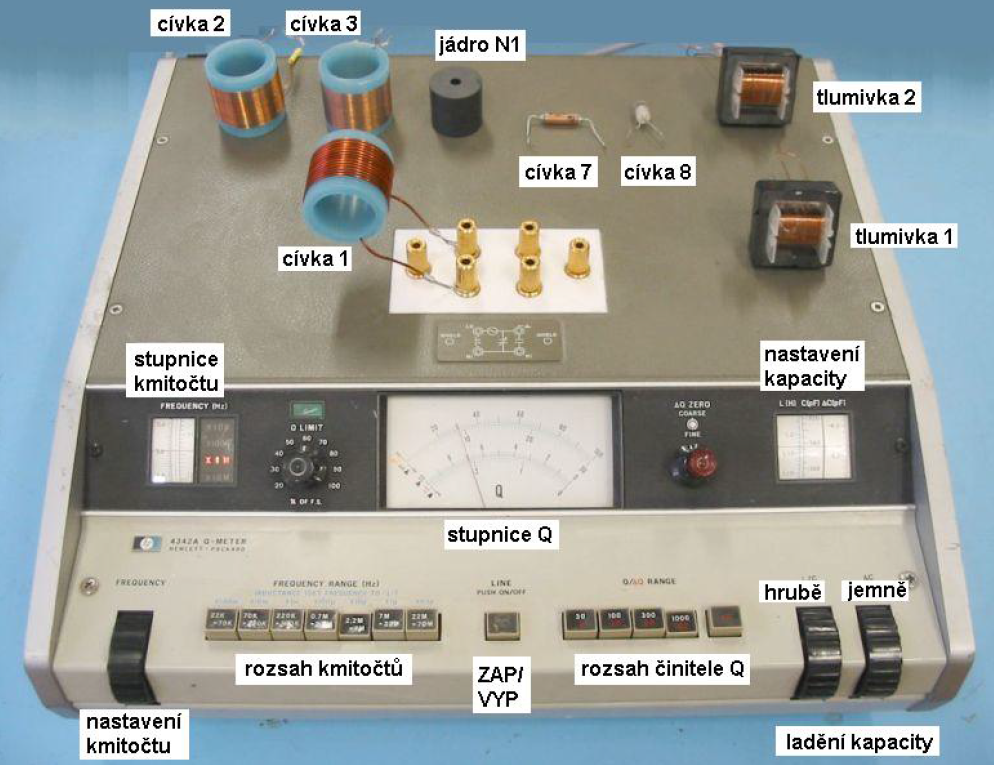
\includegraphics[width=0.9\columnwidth]{vf_civky/qmetr}
  \label{fig:vfCivky:qmetr}
\end{figure}

\section{\texorpdfstring{Neline�rn� rezistory}{Nelinearni rezistory}}

\subsection{\texorpdfstring{�vod}{Uvod}}

V praxi se nej�ast�ji setk�v�me s line�rn�mi rezistory, tj. sou��stkami, u nich� p�edpokl�d�me konstantn� velikost odporu nez�vislou na vn�j��ch podm�nk�ch aplikace, tj. nez�vislost na teplot�, frekvenci, mechanick�ch vlivech apod. Odli�uj� se v�konovou zat�itelnost�, teplotn� a frekven�n� z�vislost� podle pou�it�ch materi�l� a  technologi� v�roby, toleranc� jmenovit� hodnoty a proveden�m. P�edpoklad konstantn� velikosti odporu vyhovuje obvykle p�i aplikac�ch do frekvenc� 50~kHz a� 1~MHz (podle proveden�). Pro vy��� frekvence je nutn� uva�ovat �pln� n�hradn� sch�ma rezistoru s jeho reaktan�n�mi prvky.

Neline�rn� rezistory  jsou na rozd�l od line�rn�ch konstruov�ny tak, aby  velikost odporu byla v�razn� z�visl� na vn�j��ch podm�nk�ch, nap�. teplot� (termistory NTC, PTC) nebo p�ilo�en�mu nap�t� (varistory) a pokud mo�no nez�visela na dal��ch vlivech aplikace. Vzhledem k t�mto vlastnostem se vyu��vaj� k m��en� teploty, v obvodech pro tepelnou ochranu p��stroj�, stroj� a za��zen�, jako p�ep�ov� ochrany atd.

%---------------------------------------------
\subsection{\texorpdfstring{M��en� teplotn� z�vislosti termistor�}{Mereni teplotni zavislosti termistoru}}

\subsubsection{\texorpdfstring{�kol m��en�}{Ukol mereni}}
Zm��te z�vislost odporu 6 vzork� rezistor� a termistor� pro zm�nu teploty 20~$^\circ$C a� 120~$^\circ$C. Nam��en� z�vislosti $R= f(\vartheta)$ vyneste do grafu! Ov��te, zda dan� charakteristiky odpov�daj� teoretick�m vztah�m (line�rn� z�vislost, exponenci�ln� z�vislost apod.)

\subsubsection{\texorpdfstring{Sch�ma zapojen�}{Schema zapojeni}}

\begin{figure}[h]
  \centering
  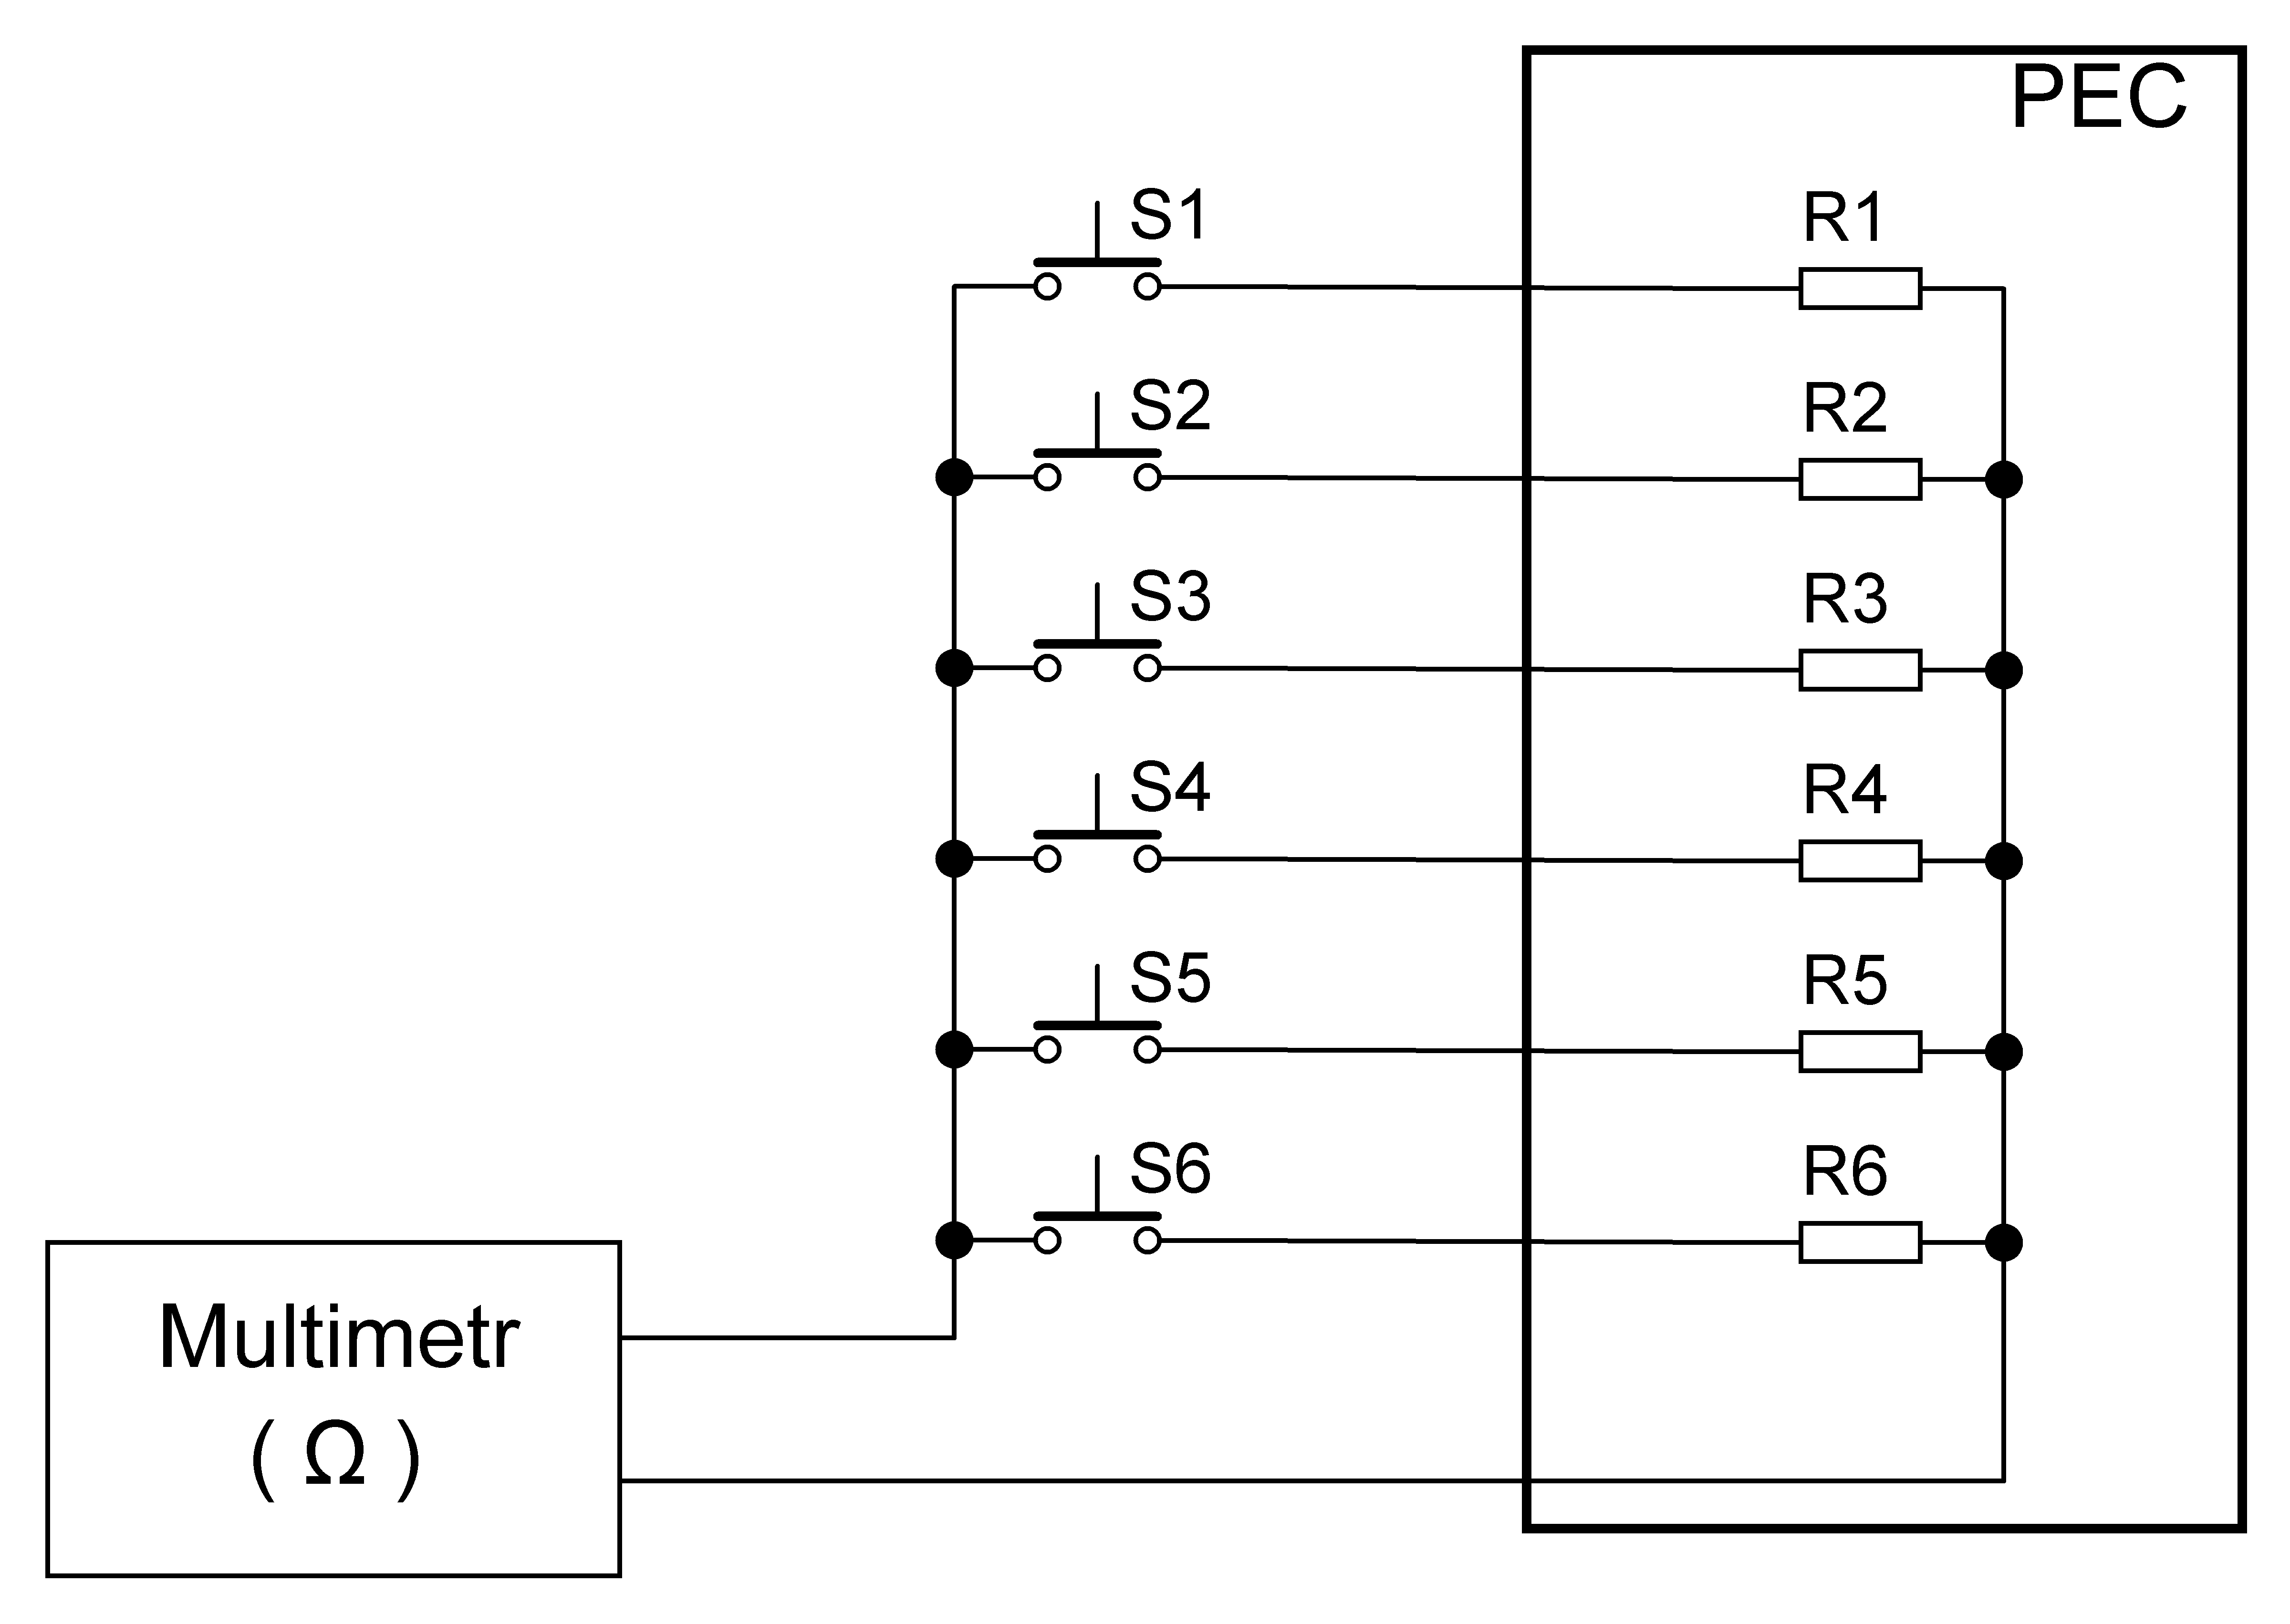
\includegraphics[width=0.5\columnwidth]{nelin_rezistory/NelinRez11}
  \label{fig:nelinRez:termistory}
\end{figure}

\subsubsection{\texorpdfstring{Postup m��en�}{Postup mereni}}

M��en� vzorky jsou um�st�ny na desti�ce v p�cce a vyvedeny na p�ep�na� m��ic�ch m�st. K m��en� teploty slou�� orienta�n� teplom�r, kter� je sou��st� konstrukce pece. Pro p�esn� m��en� vyu�ijeme Pt odporov� teplom�r s line�rn� z�vislost� odporu na teplot�. Pro odpor Pt teplom�ru uva�ujte n�sleduj�c� vztah:

\begin{equation}
R_\vartheta = R_0 \cdot \left(1 + \alpha \cdot\left(\vartheta - \vartheta_0\right)\right)
\label{eq:nelinRez:OdporNaTeplote}
\end{equation}

\begin{tabular}{ll}
 $R_0$& \ldots je odpor v $\Omega$ p�i 0~$^\circ$C, \\
 $\alpha$& \ldots je teplotn� koeficient odporu, pro platinov� teplom�r je $\alpha = 4,5 \cdot 10^{-3}$ K$^{-1}$, \\
 $\vartheta$& \ldots je teplota okol� ve $^\circ$C nebo K, \\ 
 $\vartheta_0$& \ldots je teplota ve $^\circ$C nebo K, p�i kter� byl m��en odpor $R_0$, zde 0~$^\circ$C. \\
\end{tabular}

\subsubsection{\texorpdfstring{M��en� vzorky}{Merene vzorky}}
\begin{tabular}{llll}
 1.& odporov� Pt teplom�r 100~$\Omega$ p�i 0~$^\circ$C&  4.&  rezistor uhl�kov� TR 212  4,7~k$\Omega$  \\
 2.& termistor NTC 100~$\Omega$&  5.& termistor NTC 6,8~k$\Omega$  \\
 3.& rezistor metaloxidov� TR154  6,8~k$\Omega$ &  6.& termistor PTC 60~$\Omega$  \\ 
\end{tabular}

%---------------------------------------------
\subsection{\texorpdfstring{M��en� VA charakteristiky varistor�}{Mereni VA charakteristiky varistoru}}

\subsubsection{\texorpdfstring{�kol m��en�}{Ukol mereni}}
Zm��te voltamp�rovou charakteristiku 5 vzork� varistor� pomoc� osciloskopu, kter� pracuje v re�imu x/y (sou�adnicov� zapisova�). Ov��te, zda �daje uveden� k jednotliv�m vzork�m odpov�daj� m��en�.

\subsubsection{\texorpdfstring{Sch�ma zapojen�}{Schema zapojeni}}

\begin{figure}[h]
  \centering
  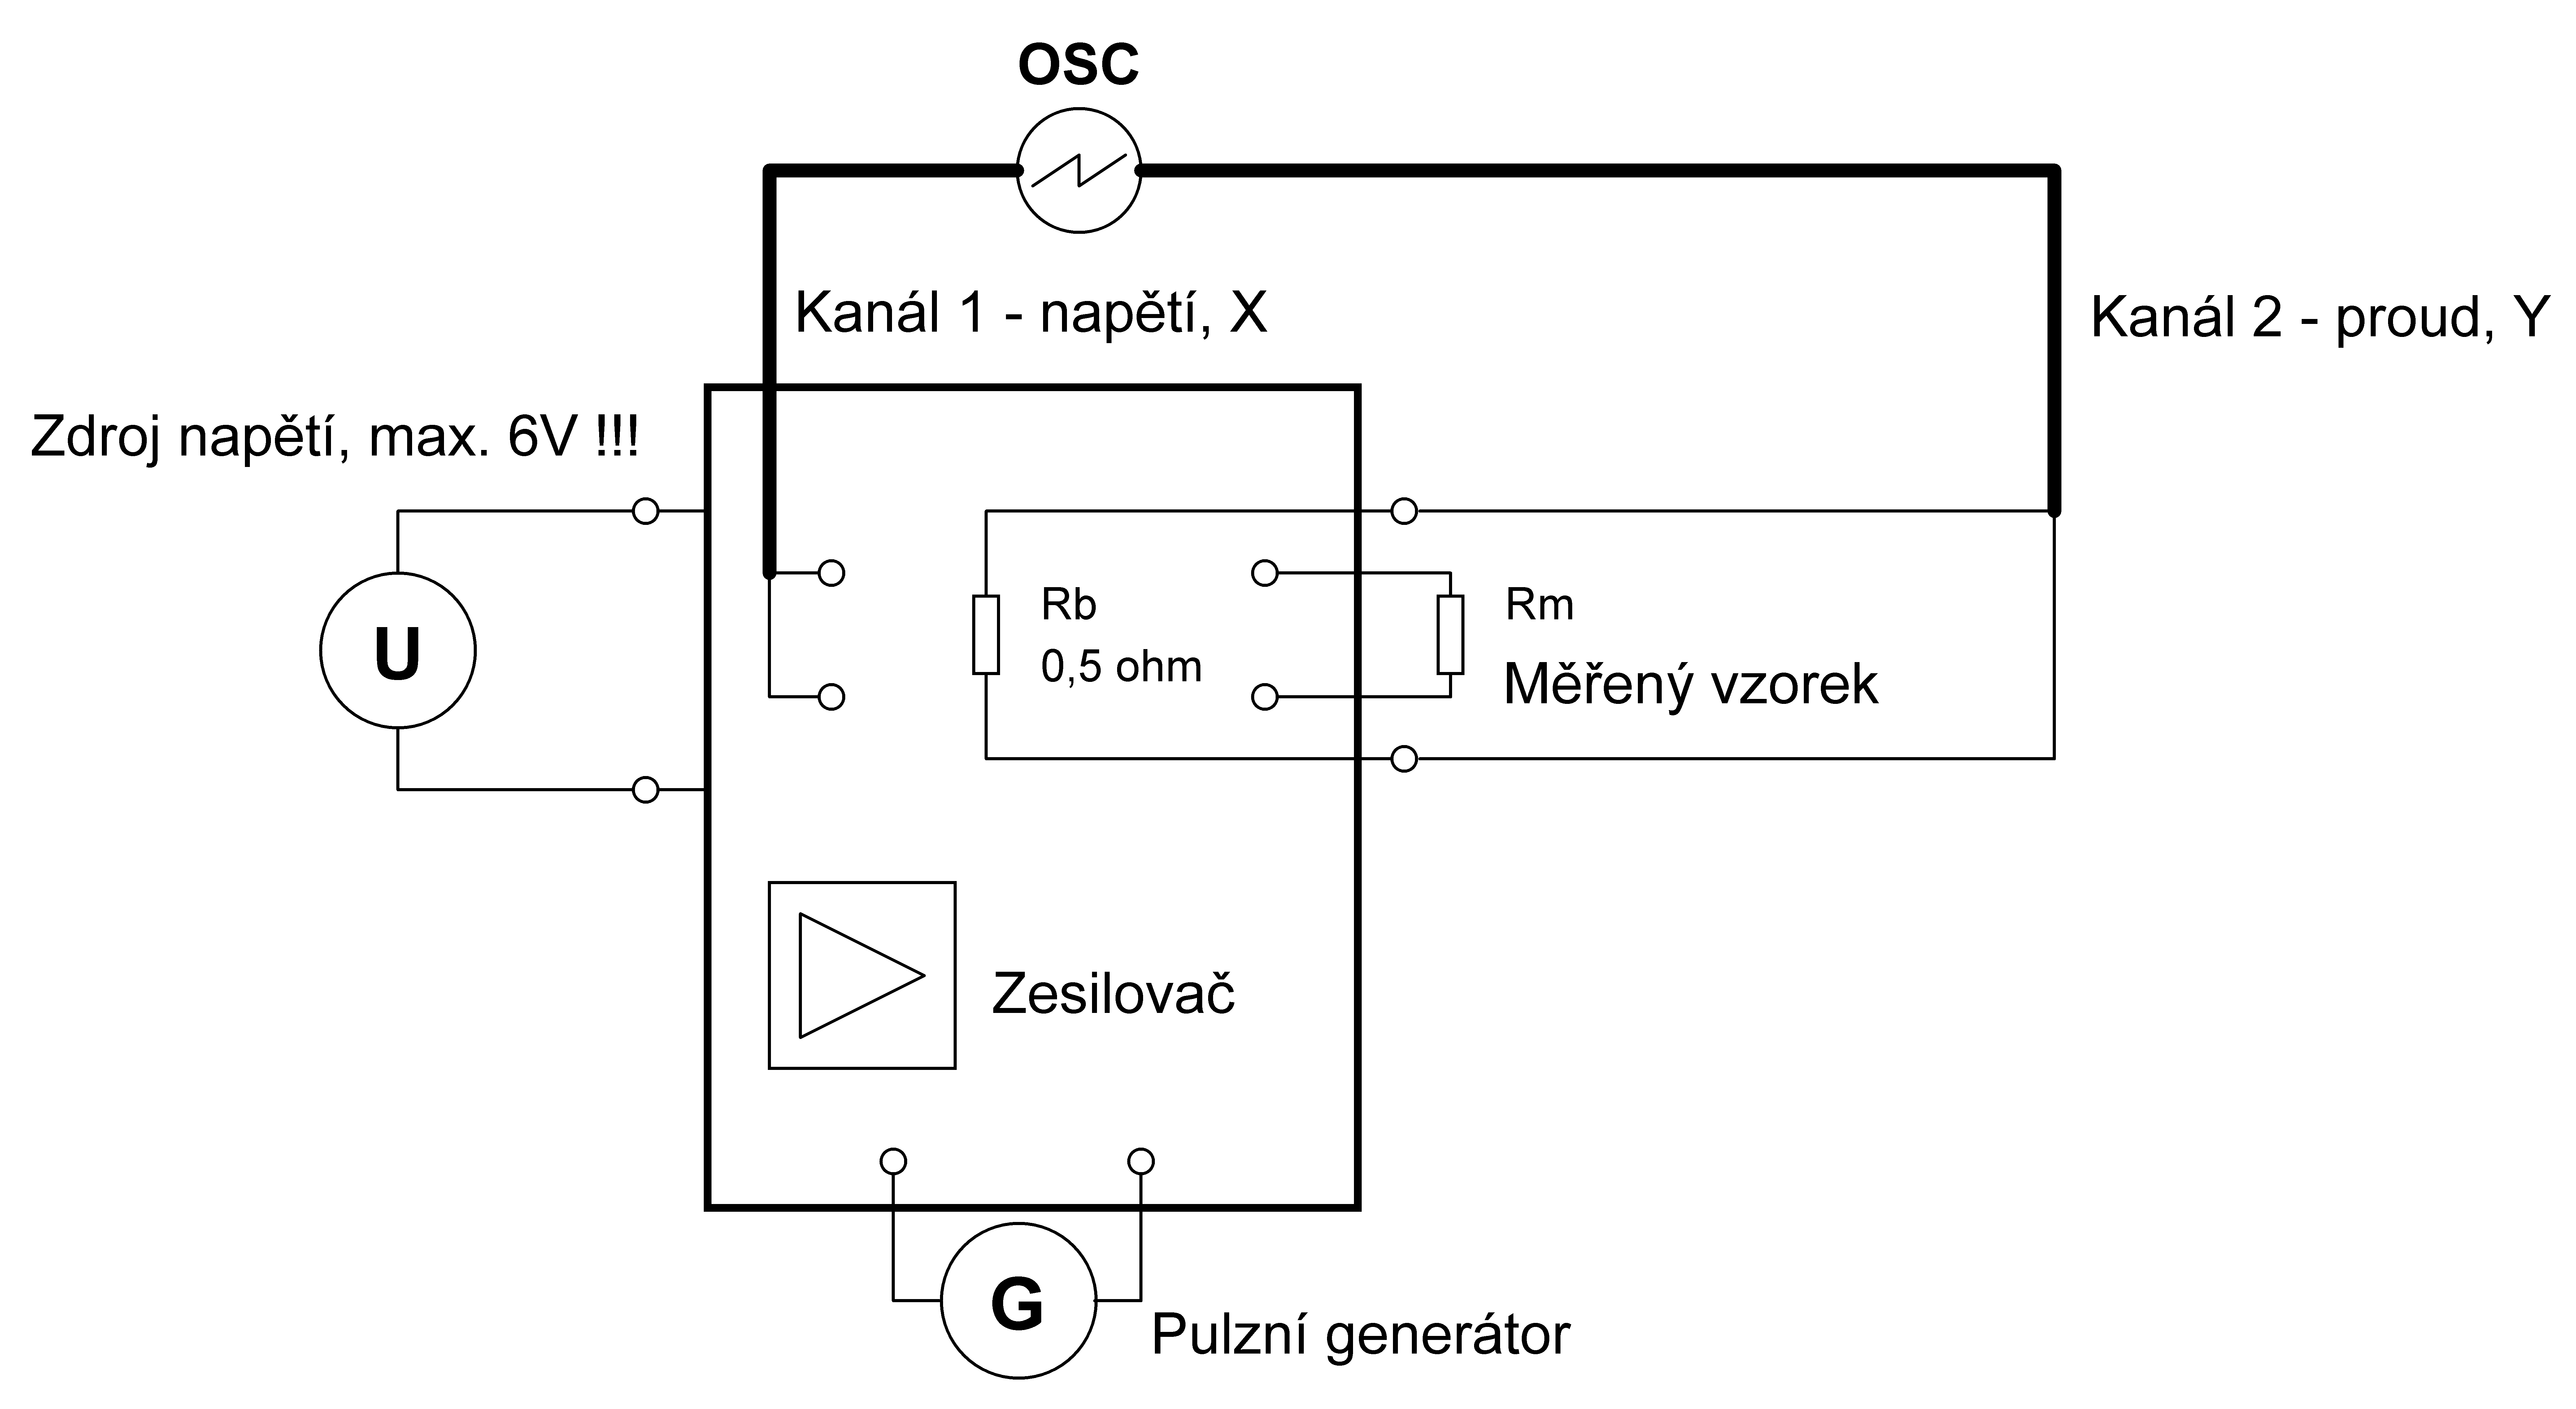
\includegraphics[width=0.8\columnwidth]{nelin_rezistory/NelinRez12}
  \label{fig:nelinRez:varistory}
\end{figure}

\subsubsection{\texorpdfstring{Postup m��en�}{Postup mereni}}

M��en� vzorek um�st�me do p��pravku. Pro m��en� pou�ijeme zdroj kr�tk�ch nap�ov�ch pulz� nastaviteln� velikosti. Pozor p�i v�m�n� vzork� -  p�ed manipulac� sni�te nap�t� na 0~V! Nap�t� na vzorku sn�m�me sondou s d�li�em 1:100 (nastaveno na osciloskopu � zkontrolovat!), proud je sn�m�n jako �bytek nap�t� na odporu 0,5~$\Omega$ nebo pomoc� proudov� sondy.  Sejmut� charakteristiky zaznamenejte na disketu v osciloskopu, p�eneste do PC a ulo�te na vhodn� pam�ov� medium pro vytisknut� do refer�tu z m��en�.

\subsubsection{\texorpdfstring{M��en� vzorky}{Merene vzorky}}
\begin{tabular}{llll}
 1.& 15D201K, 200 V, zelen�&  4.& S20K20, 40 V, velk� modr�  \\
 2.& 14D220K, 22 V, modr�&  5.& TR 152, 100 Ohm�, line�rn� rezistor  \\
 3.& 14D101K, 100 V, sv�tle modr�&  &  \\ 
\end{tabular}
\section{\texorpdfstring{Feroelektrick� kondenz�tory}{Feroelektricke kondenzatory}}

\subsection{\texorpdfstring{�vod}{Uvod}}
Kondenz�tor je sou��stka, pomoc� n� v elektrick�m obvodu realizujeme kapacitu. Podobn� jako ostatn� sou��stky vykazuje �adu vedlej��ch z�vislost� (induk�nost, s�riov� a paraleln� odpor, teplotn� a nap�ovou z�vislost). Hodnota kapacity $C$ z�vis�, jak zn�mo, na plo�e elektrod ($S$), dielektrick� konstant� ($\epsilon$) a nep��mo na vzd�lenosti elektrod ($d$). Z toho vych�zej� odli�n� konstrukce kondenz�tor� (plo�n� - nap�. sl�dov�, svitkov�, keramick�, elektrolytick�). Po�adavek na minim�ln� rozm�ry p�edpokl�d� pou�it� materi�l� dielektrika s vysokou pom�rnou dielektrickou konstantou (tzv. feroelektrika). Tyto materi�ly jsou v�ak p�i vy���ch teplot�ch zna�n� teplotn� z�visl� a jejich $\epsilon_r$ p�i vy��� teplot� rychle kles�.

\subsubsection{\texorpdfstring{Ztr�tov� �initel}{Ztratovy cinitel}}

%--------------------------------------
\newpage
\subsection{\texorpdfstring{M��en� teplotn� z�vislosti kapacity a ztr�tov�ho �initele vybran�ch vzork� kondenz�tor�}{Mereni teplotni zavislosti kapacity a ztratoveho cinitele vybranych vzorku kondenzatoru}}

\subsubsection{\texorpdfstring{�kol m��en�}{Ukol mereni}}
Zm��te z�vislost kapacity $C$ a ztr�tov�ho �initele $D$ u t�� vzork� keramick�ch kondenz�tor� s odli�n�m dielektrikem na teplot� $T$ pro teploty 20~$^\circ$C a� 120~$^\circ$C. Z�vislosti $C = f(T)$, $D = g(T)$ vyneste do grafu.

\subsubsection{\texorpdfstring{Sch�ma zapojen�}{Schema zapojeni}}

\begin{figure}[h]
  \centering
  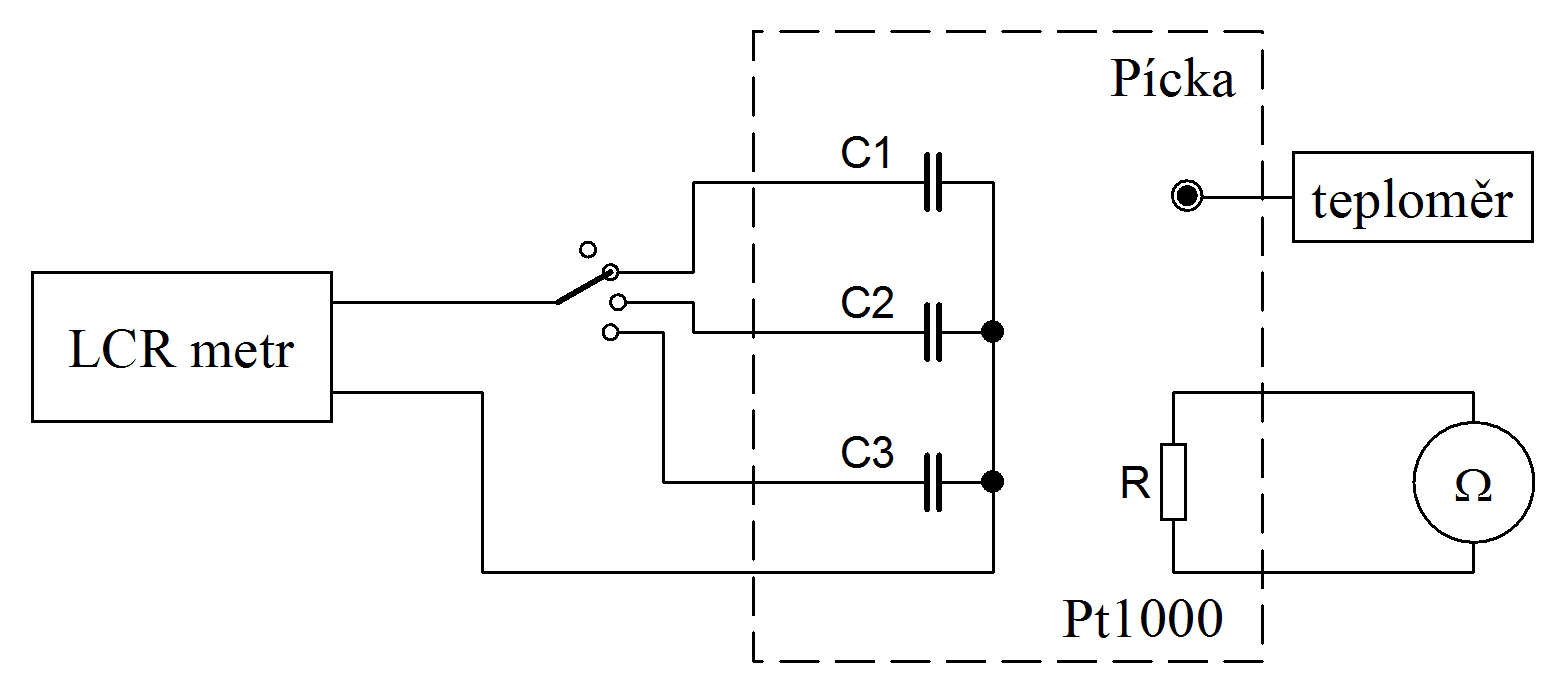
\includegraphics[width=0.7\columnwidth]{feroel_kondenzatory/feroelKond1}
  \label{fig:feroelKond:feroelKond1}
\end{figure}

\subsubsection{\texorpdfstring{Postup m��en�}{Postup mereni}}
M��en� vzorky jsou um�st�ny na desti�ce v p�cce a vyvedeny na p�ep�na� m��ic�ch m�st. K m��en� teploty slou�� orienta�n� dotykov� teplom�r zasazen� do m�rn� j�mky na t�lese p�cky. Kapacitu vzork� a ztr�tov� �initel m���me RLC metrem. K p�esn�mu zm��en� teploty slou�� odporov� teplom�r (�idlo Pt1000, $R_0 = 1008$~$\Omega$ p�i 0~$^\circ$C, $\alpha = 4,5 \cdot 10^{-3}$ K$^{-1}$), jeho� odpor m���me pomoc� multimetru. Teplotu vypo�teme z �daj� uveden�ch v��e v n�vodu a za p�edpokladu linearn� z�vislosti mezi hodnotou odporu a teplotou:
 
\begin{equation}
R_\vartheta = R_0 \cdot \left(1 + \alpha \cdot\left(\vartheta - \vartheta_0\right)\right)
\label{eq:feroelKond:OdporNaTeplote}
\end{equation}

\begin{tabular}{ll}
 $R_0$& \ldots je odpor v $\Omega$ p�i 0~$^\circ$C, \\
 $\alpha$& \ldots je teplotn� koeficient odporu, pro platinov� teplom�r je $\alpha = 4,5 \cdot 10^{-3}$ K$^{-1}$, \\
 $\vartheta$& \ldots je teplota okol� ve $^\circ$C nebo K, \\ 
 $\vartheta_0$& \ldots je teplota ve $^\circ$C nebo K, p�i kter� byl m��en odpor $R_0$, zde 0~$^\circ$C. \\
\end{tabular}

\subsubsection{\texorpdfstring{M��en� vzorky}{Merene vzorky}}
\begin{tabular}{ll}
 1.& keramick� kondenz�tor 100 nF, hmota X7R \\
 2.& keramick� kondenz�tor 150 nF, hmota Z5U \\
 3.& keramick� kondenz�tor 150 nF, hmota Y5VV \\ 
\end{tabular}

%--------------------------------------
\newpage
\subsection{\texorpdfstring{M��en� nap�ov� z�vislosti kapacity vybran�ch vzork� kondenz�tor�}{Mereni napetove zavislosti kapacity vybranych vzorku kondenzatoru}}

\subsubsection{\texorpdfstring{�kol m��en�}{Ukol mereni}}
Zm��te z�vislost kapacity t�� vzork� keramick�ch kondenz�tor� na velikosti p�ilo�en�ho stejnosm�rn�ho nap�t�. Z�vislost $C = f(U)$ vyneste do grafu.

\subsubsection{\texorpdfstring{Sch�ma zapojen�}{Schema zapojeni}}

\begin{figure}[h]
  \centering
  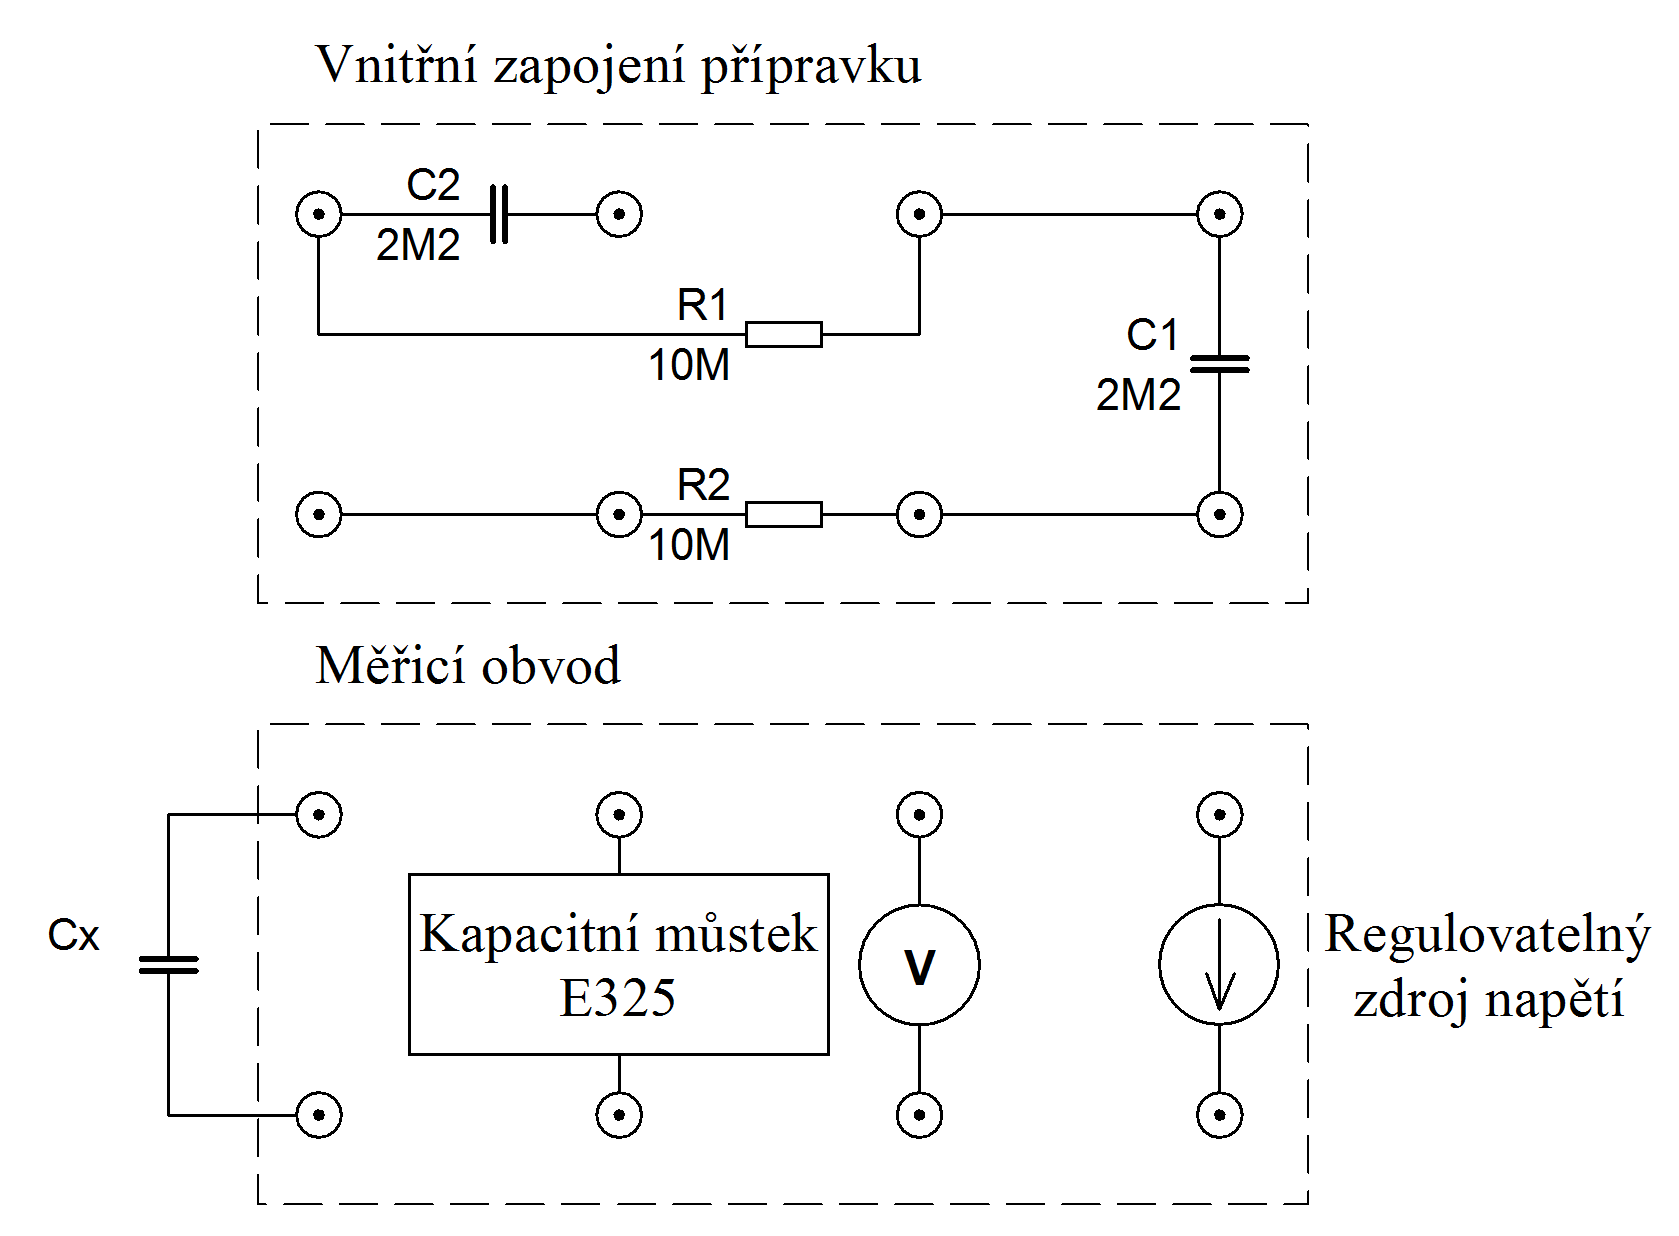
\includegraphics[width=0.7\columnwidth]{feroel_kondenzatory/feroelKond2}
  \label{fig:feroelKond:feroelKond2}
\end{figure}

\subsubsection{\texorpdfstring{Postup m��en�}{Postup mereni}}
M��en� vzorky postupn� zapojujeme na svorky \uv{$C_X$} m��ic�ho p��pravku, kter� umo��uje odd�len� p�ilo�en�ho nap�t� (z bateriov�ho DC zdroje) a m��ic�ho mal�ho st��dav�ho nap�t�, kter� vyu��v�me pro m��en� kapacity. P�i m��en� db�me na to, aby nebylo p�ekro�eno jmenovit� provozn� nap�t� vzorku.

\subsubsection{\texorpdfstring{M��en� vzorky}{Merene vzorky}}
\begin{tabular}{ll}
 1.& keramick� kondenz�tor TK666, 40 V,100 nF, hmota Supermit (kotou�ov�, hn�d�) \\
 2.& keramick� kondenz�tor 4H30, 40 V, 33 nF (zelen�) \\
 3.& svitkov� kondenz�tor CF2, 63 V, 100 nF, tereftal�tov� (�lut�) \\ 
\end{tabular}

%--------------------------------------
\newpage
\subsection{\texorpdfstring{M��en� uvoln�n� n�boje feroelektrick�ho kondenz�toru}{Mereni uvolneni naboje feroelektrickeho kondenzatoru}}
V objemu dielektrika feroelektrick�ho kondenz�toru je obecn� v�dy v�z�n mal� zbytkov� n�boj $Q_1$. Jemu odpov�d� n�zk� nap�t� $U_1$ na svork�ch kondenz�toru, kter� je d�no rovnic�: 

\begin{equation}
U_1 = \frac{Q_1}{C_1}
\label{eq:feroelKond:NapetiNabojKapacita}
\end{equation}

P�i zv��en� teploty doch�z� u feroelektrik k v�razn�mu zmen�en� jejich kapacity (z $C_1$ na $C_2$) d�ky zmen�en� relativn� permitivity z $\epsilon_{r1}$ na $\epsilon_{r2}$. Aby z�stal zachov�n zbytkov� n�boj ($Q_1 = Q_2$), mus� na kondenz�toru v�razn� vzr�st nap�t� ($U_2$). V ide�ln�m p��pad� plat�, �e vzr�st nap�t� ($U_2/U_1$) je roven zm�n� permitivity ($\epsilon_{r1}/\epsilon_{r2}$).

\subsubsection{\texorpdfstring{�kol m��en�}{Ukol mereni}}
Ov��te uvoln�n� elektrick�ho n�boje u p�edlo�en�ho vzorku kondenz�toru z feroelektrick�ho materi�lu.

\subsubsection{\texorpdfstring{Postup m��en�}{Postup mereni}}
Kondenz�tor p�ipojen� k elektrostatick�mu voltmetru nabijte na pln� nap�t� bateriov�ho zdroje (asi 120~V). Kondenz�tor vybijte a po chv�li oh�ejte v olejov� l�zni na cca 150~$^\circ$C. Ode�t�te maxim�ln� nap�t� kondenz�toru.

\section{\texorpdfstring{Vlastnosti kondenz�tor� a rezistor� p�i kmito�tech do 1~MHz }{Vlastnosti kondenzatoru a rezistoru pri kmitoctech do 1 MHz}}

\subsection{\texorpdfstring{�vod}{Uvod}}

%---------------------------------------------
\newpage
\subsection{\texorpdfstring{Kmito�tov� z�vislost rezistor�}{Kmitoctova zavislost rezistoru}}

\subsubsection{\texorpdfstring{�kol m��en�}{Ukol mereni}}
Pro zadan� vzorky rezistor� zm��te z�vislost impedance (absolutn� hodnoty $\vert Z \vert$, f�ze $\varphi$) nebo jin�ch ekvivalentn�ch slo�ek ($R$, $X$) vyjad�uj�c�ch komplexn� impedanci rezistoru na kmito�tu. Nam��en� hodnoty vyneste do grafu, volte vhodn� (logaritmick�) m���tko na kmito�tov� ose! 

\subsubsection{\texorpdfstring{Sch�ma zapojen�}{Schema zapojeni}}

\subsubsection{\texorpdfstring{Postup m��en�}{Postup mereni}}

M��en� prove�te v rozsahu kmito�t� od cca 50~Hz a� do 1~MHz s pou�it�m p��stroje HP~4284A. Volte vhodn� krok, abyste pokryli rovnom�rn� v�echny  m��en� ��dy (Hz, kHz, MHz). Pro  vyn�en� v logaritmick� m���tku je vhodn� krok 1-2-5-10  nebo 1-3-10. P��stroj umo��uje nastaven� kmito�tu jen s ur�it�m krokem z p�edvolen� �ady hodnot. Dbejte, aby p�i upnut� sou��stek byl minimalizov�n vliv jejich p��vod� (tj. p�ipojovat kr�tk�mi p��vody). 

U odpor� tzv. mal�ch hodnot (��dov� jednotky a� des�tky $\Omega$) vyhodno�te s�riovou induk�nost $L_S$ (z m��en� impedance), u odpor� tzv. velk�ch hodnot (��dov� od k$\Omega$ v��e) paraleln� kapacitu $C_P$. Pov�imn�te si t� chov�n� vykompenzovan�ch odpor� s hodnotami rezistivity kolem 300~$\Omega$. P�i z�v�re�n�m hodnocen� se v�nujte i vlivu konstrukce rezistor� na jejich chov�n�. 

\subsubsection{\texorpdfstring{M��en� vzorky}{Merene vzorky}}
\begin{tabular}{lll}
 1.& 10~$\Omega$/ 330~$\Omega$/ 10~k$\Omega$& rezistor metalizovan�, 0,6 W, velikost 0207  \\
 2.& 10~$\Omega$/ 330~$\Omega$/ 10~k$\Omega$& rezistor metalizovan�, 2 W, velikost 0414  \\
 3.& 10~$\Omega$/ 330~$\Omega$/ 10~k$\Omega$& rezistor dr�tov�, 5 W, keramick� pouzdro  \\ 
\end{tabular}

%---------------------------------------------
\subsection{\texorpdfstring{Kmito�tov� z�vislost kondenz�tor�}{Kmitoctova zavislost kondenzatoru}}

\subsubsection{\texorpdfstring{�kol m��en�}{Ukol mereni}}
Pro zadan� vzorky kondenz�tor� zm��te z�vislost impedance (absolutn� hodnoty $\vert Z \vert$, f�ze $\varphi$) nebo kapacity $C$ a ztr�tov�ho �initele $D$ na kmito�tu. Nam��en� hodnoty vyneste do grafu, volte vhodn� (logaritmick�) m���tko na kmito�tov� ose!

\subsubsection{\texorpdfstring{Sch�ma zapojen�}{Schema zapojeni}}

\subsubsection{\texorpdfstring{Postup m��en�}{Postup mereni}}

M��en� prove�te v rozsahu kmito�t� od cca 50~Hz a� do 1~MHz s pou�it�m p��stroje HP~4284A. Volte vhodn� krok, abyste pokryli rovnom�rn� v�echny  m��en� ��dy (Hz, kHz, MHz). Pro  vyn�en� v logaritmick� m���tku je vhodn� krok 1-2-5-10  nebo 1-3-10. P��stroj umo��uje nastaven� kmito�tu jen s ur�it�m krokem z p�edvolen� �ady hodnot. Dbejte, aby p�i upnut� sou��stek byl minimalizov�n vliv jejich p��vod� (tj. p�ipojovat kr�tk�mi p��vody). Pov�imn�te si v�razn� induktivn� slo�ky u svitkov�ch kondenz�tor�. Pokuste se porovnat jednotliv� technologie kondenz�tor� mezi sebou z pohledu jejich frekven�n� charakteristiky.

\subsubsection{\texorpdfstring{M��en� vzorky}{Merene vzorky}}
\begin{tabular}{lll}
 1.& 1 nF/10 nF/68 nF& miniaturn� keramick�  \\
 2.& 10 nF& plastov� s radi�ln�mi v�vody WIMA  \\
 3.& 10 nF& plastov� s axi�ln�mi v�vody   \\ 
 4.& 330 $\mu$F/25 V& elektrolytick� hlin�kov�  \\
 5.& 22 $\mu$F/10 V& elektrolytick� tantalov�   \\ 
\end{tabular}

%--------------------------------------
\subsection{\texorpdfstring{Obr�zkov� p��loha}{Obrazkova priloha}}
\section{\texorpdfstring{Vlastnosti kondenz�tor� a rezistor� p�i kmito�tech nad 1~MHz }{Vlastnosti kondenzatoru a rezistoru pri kmitoctech nad 1 MHz}}

\subsection{\texorpdfstring{�vod}{Uvod}}

Rezistory a kapacitory nejsou ide�ln� sou��stky, tak�e mimo svou dominantn� vlastnost (odpor, kapacita) vykazuj� je�t� parazitn� vlastnosti (induk�nost, kapacitu, s�riov� a paraleln� odpor). Ty ovliv�uj� jejich vlastnosti, a to p�edev��m v obvodech s vy���mi frekvencemi. M��en� slou�� k ov��en� kmito�tov�ho rozsahu, v n�m� sou��stka vykazuje p�ev�n� svou dominantn� vlastnost. Vlastnosti jednotliv�ch vzork� z�vis� na jejich rozm�rech, pou�it�ch materi�lech, technologii v�roby atd.

%---------------------------------------------
\subsection{\texorpdfstring{Kmito�tov� z�vislost rezistor�}{Kmitoctova zavislost rezistoru}}

\subsubsection{\texorpdfstring{�kol m��en�}{Ukol mereni}}
Pro zadan� vzorky rezistor� zm��te z�vislost absolutn� hodnoty impedance a f�ze ($\left|Z\right|$, $\varphi$) na kmito�tu. Nam��en� hodnoty vyneste do grafu. V z�v�ru diskutujte vliv hodnoty a technologie rezistoru na nam��en� frekven�n� charakteristiky.

\subsubsection{\texorpdfstring{Postup m��en�}{Postup mereni}}

M��en� prove�te v rozsahu frekvenc� 1 MHz a� 100 MHz s pou�it�m p��stroje Agilent E5062A. Vyhodno�te, jak se jednotliv� vzorky projevuj� v z�vislosti na jejich hodnot� a technologii. Zaznamenejte rezonan�n� frekvence jednotliv�ch sou��stek.

\subsubsection{\texorpdfstring{M��en� vzorky}{Merene vzorky}}
\begin{tabular}{lll}
 1.& 10~$\Omega$/ 330~$\Omega$/ 10~k$\Omega$& rezistor metalizovan�, 0,6 W, velikost 0207  \\
 2.& 10~$\Omega$/ 330~$\Omega$/ 10~k$\Omega$& rezistor metalizovan�, 2 W  \\
 3.& 10~$\Omega$/ 330~$\Omega$/ 10~k$\Omega$& rezistor dr�tov�, 5 W  \\ 
\end{tabular}

%---------------------------------------------
\subsection{\texorpdfstring{Kmito�tov� z�vislost kondenz�tor�}{Kmitoctova zavislost kondenzatoru}}

\subsubsection{\texorpdfstring{�kol m��en�}{Ukol mereni}}
Pro zadan� vzorky kondenz�tor� zm��te z�vislost kapacity a ztr�tov�ho �initele ($C$, $tg\delta$) na kmito�tu. Nam��en� hodnoty vyneste do grafu. V z�v�ru diskutujte vliv technologie kondenz�toru na nam��en� frekven�n� charakteristiky.

\subsubsection{\texorpdfstring{Postup m��en�}{Postup mereni}}

M��en� prove�te v rozsahu frekvenc� 1~MHz a� 100~MHz s pou�it�m p��stroje Agilent E5062A. Vyhodno�te, jak se jednotliv� vzorky projevuj� v z�vislosti na jejich technologii. Zaznamenejte rezonan�n� frekvence jednotliv�ch sou��stek.

\subsubsection{\texorpdfstring{M��en� vzorky}{Merene vzorky}}
\begin{tabular}{llll}
 1.& Elektrolytick� kondenz�tor hlin�kov�, 330 $\mu$F/ 25 V &  5.& Keram. kondenz�tor, 1 nF  \\
 2.& Elektrolytick� kondenz�tor tantalov�, 22 $\mu$F/ 10 V & 6.& Keram. kondenz�tor, 10 nF  \\ 
 3.& Foliov� kondenz�tor radi�ln�, 10 nF/ 100 V  & 7.& Keram. kondenz�tor, 68 nF  \\ 
 4.& Foliov� kondenz�tor axi�ln�, 10 nF/ 100 V  && \\
\end{tabular}

%---------------------------------------------
\subsection{\texorpdfstring{M��en� p��strojem Agilent E5062A}{Mereni pristrojem Agilent E5062A}}

\subsubsection{\texorpdfstring{Sch�ma zapojen�}{Schema zapojeni}}

\begin{figure}[h]
  \centering
  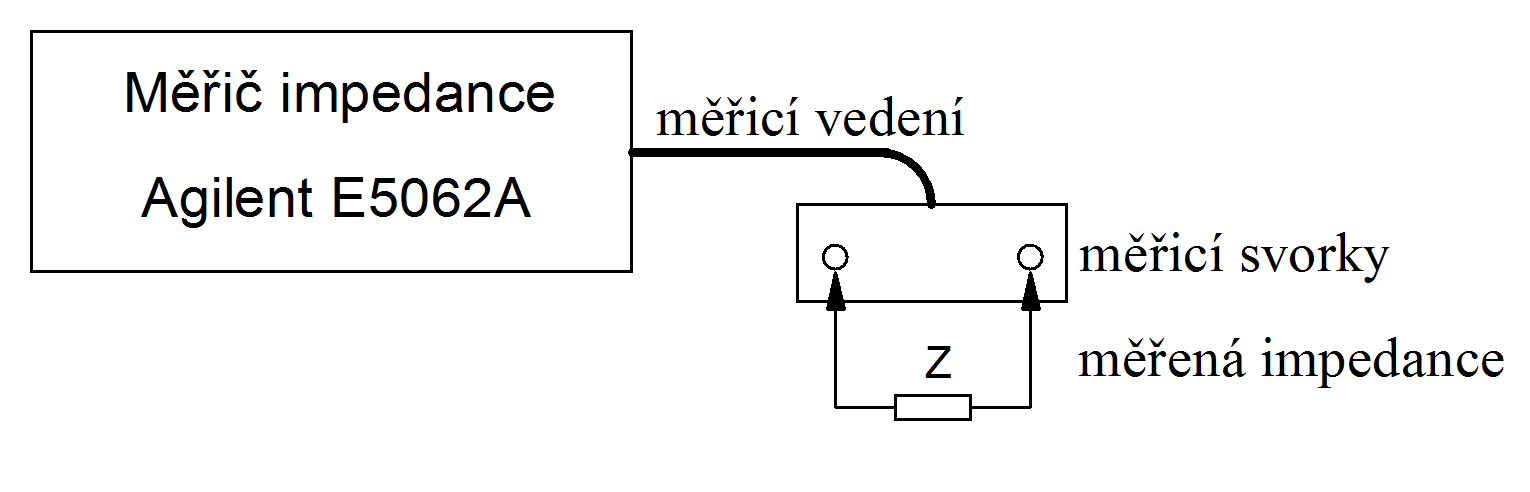
\includegraphics[width=0.2\columnwidth]{rc_nad_1MHz/RCmer21}
  \label{fig:rcNad1MHz:schemaZap}
\end{figure}

\subsubsection{\texorpdfstring{Postup m��en�}{Postup mereni}}
Bez zalo�en�ho vzorku na za��tku m��en� zkontrolujeme kalibraci p��stroje � kurzor ukazuje na prav� okraj kru�nice na displeji (poloha 3 hodiny). Pokud ne, je t�eba kalibrovat:

\textbf{\uv{Save/Recall} / \uv{Recall/State} / \uv{File Dialog} / \uv{Lab.sta} / \uv{Open}} 

\noindent Zalo��me vzorek do �elist�. Tla��tky \textbf{START} a \textbf{STOP} lze zadat z kl�vesnice po��te�n� a kone�nou frekvenci m��en�. Body k�ivky m��eme ��st manu�ln� nebo zaznamenat celou k�ivku automaticky na pam�ov� medium.

\subsubsection*{\texorpdfstring{Manu�ln� nastaven� frekvence:}{Manualni nastaveni frekvence}}
Aktu�ln� frekvenci m��eme nastavit p�i nastaven� volby Marker /Marker1. Frekvenci nastavujeme ot��en�m voli�e nebo z kl�vesnice. Na displeji je mo�n� ode��st �daje v n�sleduj�c�m po�ad�: frekvence ($f$), odpor ($R$), reaktance ($X$), induk�nost ($L$) nebo kapacita ($C$) podle znamenka reaktance.

\subsubsection*{\texorpdfstring{Automatick� m��en�:}{Automaticka mereni}}
M��en� prob�h� kontinu�ln�. Data zapisujeme na flash disk. Postupn� vol�me:

\textbf{\uv{Save/Recall} / \uv{Save Trace Data}}

\noindent \textbf{Nezapome�te zvolit vhodn� ulo�i�t�!!!}. Jm�no souboru je nutn� zadat z kl�vesnice. Stiskem \textbf{\uv{Save}} se data ulo�� ve fotm�tu CSV. Form�t ukl�d�n� je CSV. Tento form�t soubor� lze b�n� editovat softwary Excel, Matlab apod.

\subsubsection{\texorpdfstring{Smith�v diagram}{Smithuv diagram}}
\begin{multicols}{2}

\begin{centering}
  \includegraphics[width=0.8\columnwidth]{rc_nad_1MHz/smithDiag}
  \label{fig:rcNad1MHz:smithDiag}
\end{centering}

Smith�v diagram graficky zn�zor�uje z�vislost �initele odrazu na zakon�ovac� impedanci veden� $Z$.

\begin{equation}
\rho = \frac{Z-Z_0}{Z+Z_0}
\label{eq:rcNad1MHz:cinitelOdrazu}
\end{equation}

P�i zn�m�m �initeli odrazu $\rho$ (lze zm��it) a zn�m� charakteristick� impedanci veden� $Z_0$ lze ze Smithova diagramu ur�it zakon�ovac� impedanci veden�.
\end{multicols}
\section{\texorpdfstring{Osazov�n� DPS}{Osazovani DPS}}

\subsection{\texorpdfstring{�vod}{Uvod}}
P�jen� je zp�sob spojov�n� dvou kovov�ch materi�l� pomoc� jin�ho roztaven�ho kovov�ho materi�lu, tzv. p�jky. Teplota t�n� p�jky je obvykle mnohem ni���, ne� je tomu u p�jen�ch materi�l�, proto p�i p�jen� nedoch�z� k taven� spojovan�ch sou��st�. V elektrotechnice se pro vytv��en� vodiv�ch spoj� pou��vaj� t�m�� v�hradn� tzv. m�kk� p�jky. To jsou materi�ly, u nich� je teplota t�n� ni��� ne� 400~$^\circ$C. Lze se setkat se dv�ma skupinami pou��van�ch slitin:
P�jky obsahuj�c� olovo � jsou zalo�eny na slitin� Sn-Pb. Jejich v�hodou je n�zk� bod t�n�, kter� je pouze 183~$^\circ$C. Nev�hodou je obsah olova, kter� je toxick�. Pou��v�n� t�chto p�jek je omezeno sm�rnic� RoHS pouze pro speci�ln� ��ely.
P�jky bez olova � jde o slitiny c�nu a dal��ch kov�, jako nap��klad Ag, Zn, Cu a dal��. Teplota t�n� je vy��� ne� u p�jek s olovem a jej� obvykl� hodnota je 217~$^\circ$C.
Tavidla jsou nekovov� materi�ly usnad�uj�c� p�jen�. Zlep�uj� sm��ivost dan�ch materi�l� p�jkou a br�n� oxidaci roztaven� p�jky. Nej�ast�ji se pro tento ��el pou��v� kalafuna.

%--------------------------------------
\newpage
\subsection{\texorpdfstring{Osazov�n� desky plo�n�ho spoje}{Mereni frekvencni zavislosti cinitele previseni Q}}

\subsubsection{\texorpdfstring{�kol m��en�}{Ukol mereni}}
Osa�te p�ipraven� plo�n� spoj a pomoc� p��pravku ov��te jeho funk�nost.

\subsubsection{\texorpdfstring{Popis zapojen�}{Popis zapojeni}}
Sch�ma zapojen� osazovan�ho obvodu je na obr�zku \ref{fig:osDPS:schemaZap}. Jedn� se o akustickou signalizaci, kter� m� upozornit �idi�e na nutnost rozsv�tit sv�tla. Nap�jec� nap�t� a logick� sign�ly sv�tel jsou p�iv�d�ny na konektor K1. Reproduktor je p�ipojen mezi v�vody J1 a J2. Ke generov�n� obd�ln�kov�ho sign�lu pro reproduktor je pou�it integrovan� obvod �asova�e TS555. Sign�l je odeb�r�n proti zemi z v�stupu Q. Hodnotu periody generovan�ho sign�lu lze ovlivnit zm�nou �asov� konstanty RC �l�nku, kter� je slo�en z rezistoru R1 a kondenz�toru C3.
�innost �asova�e je ovliv�ov�na logickou �rovn� na vstupu R. Pokud je zde n�zk� �rove�, pak je �asova� vy�azen z �innosti. Po p�ipojen� nap�jec�ho nap�t� (oto�en� kl��ku automobilu) je na tomto vstupu nap�t� bl�zk� 0 V d�ky rezistoru R2, kter� je p�ipojen proti plovouc� zemi (bude vysv�tleno d�le). �asova� tedy nekmit�, dokud nap�t� na tomto vstupu nedos�hne po�adovan� vysok� �rovn�. Nap�t� je na vstup p�iv�d�no p�es diodu D5 z kondenz�toru C2, kter� je pozvolna nab�jen z nap�jec�ho zdroje p�es diodu D3 a rezistor R4. Volbou hodnot rezistoru R4 a kondenz�toru C2 tak ovliv�ujeme d�lku �asov� prodlevy p�ed spu�t�n�m akustick� signalizace po zapnut� p��pravku.
Nap�jec� nap�t� pro �asova� je vyvedeno mezi uzly V+ a GND. GND je zde zna�ena plovouc� zem, co� je uzel, kter� je odd�len od skute�n� zem� nap�jec�ho zdroje rezistorem R5. P�iveden�m ur�it�ho nap�t� na tento rezistor p�es diody D1 nebo D2 sn��me o jeho hodnotu nap�jec� nap�t� �asova�e. Pokud je toto nap�t� rovno nap�t� zdroje nap�jen�, pak je nap�jec� nap�t� �asova�e rovno nule a obvod op�t nem��e kmitat.

\subsubsection{\texorpdfstring{Postup p�jeni}{Postup pajeni}}
Desku plo�n�ho spoje osazujeme dle obr�zku \ref{fig:osDPS:schemaPokl}, kter� ukazuje pozice sou��stek ze strany sou��stek (druh� strana se naz�v� strana plo�n�ho spoje a jsou na n� vyleptan� vodiv� trasy). Db�me na polaritu diod a elektrolytick�ch kondenz�tor� a tak� na spr�vn� nato�en� pouzdra integrovan�ho obvodu, kter� je vyzna�eno kl��em (symbol na pouzd�e � te�ka, v��ez apod.). P�i osazov�n� je vhodn� za��t sou��stkami s n�zk�m profilem (v��kou). P�jen� bude jednodu���, pokud si desku plo�n�ho spoje upevn�me do dr��ku.
\noindent
Spoje p�j�me n�sleduj�c�m posupem:
\begin{enumerate}
	\item P�je�ku dr��me v jedn� ruce, trubi�kovou p�jku ve druh�.
	\item P�ilo��me p�je�ku ke spoji a za�neme jej proh��vat (p��padn� je�t� p�edt�m namo��me p�je�ku do kalafuny).
	\item Dotkneme se p�jkou proh��van�ho spoje � trocha p�jky se roztav� a z�stane na p�je�ce a spoji. P�je�kou st�le proh��v�me spoj!!!
	\item Pot� co se p�jka rozte�e po spoji, p�je�ku odejmeme. V�dy se sna��me, zkr�tit dobu p�jen� na minimum.
\end{enumerate}
V�sledn� p�jen� spoj by m�l m�t vzhled sopky.
\newpage
\subsubsection{\texorpdfstring{Sch�ma zapojen�}{Sch�ma zapojen�}}

\begin{figure}[h]
  \centering
  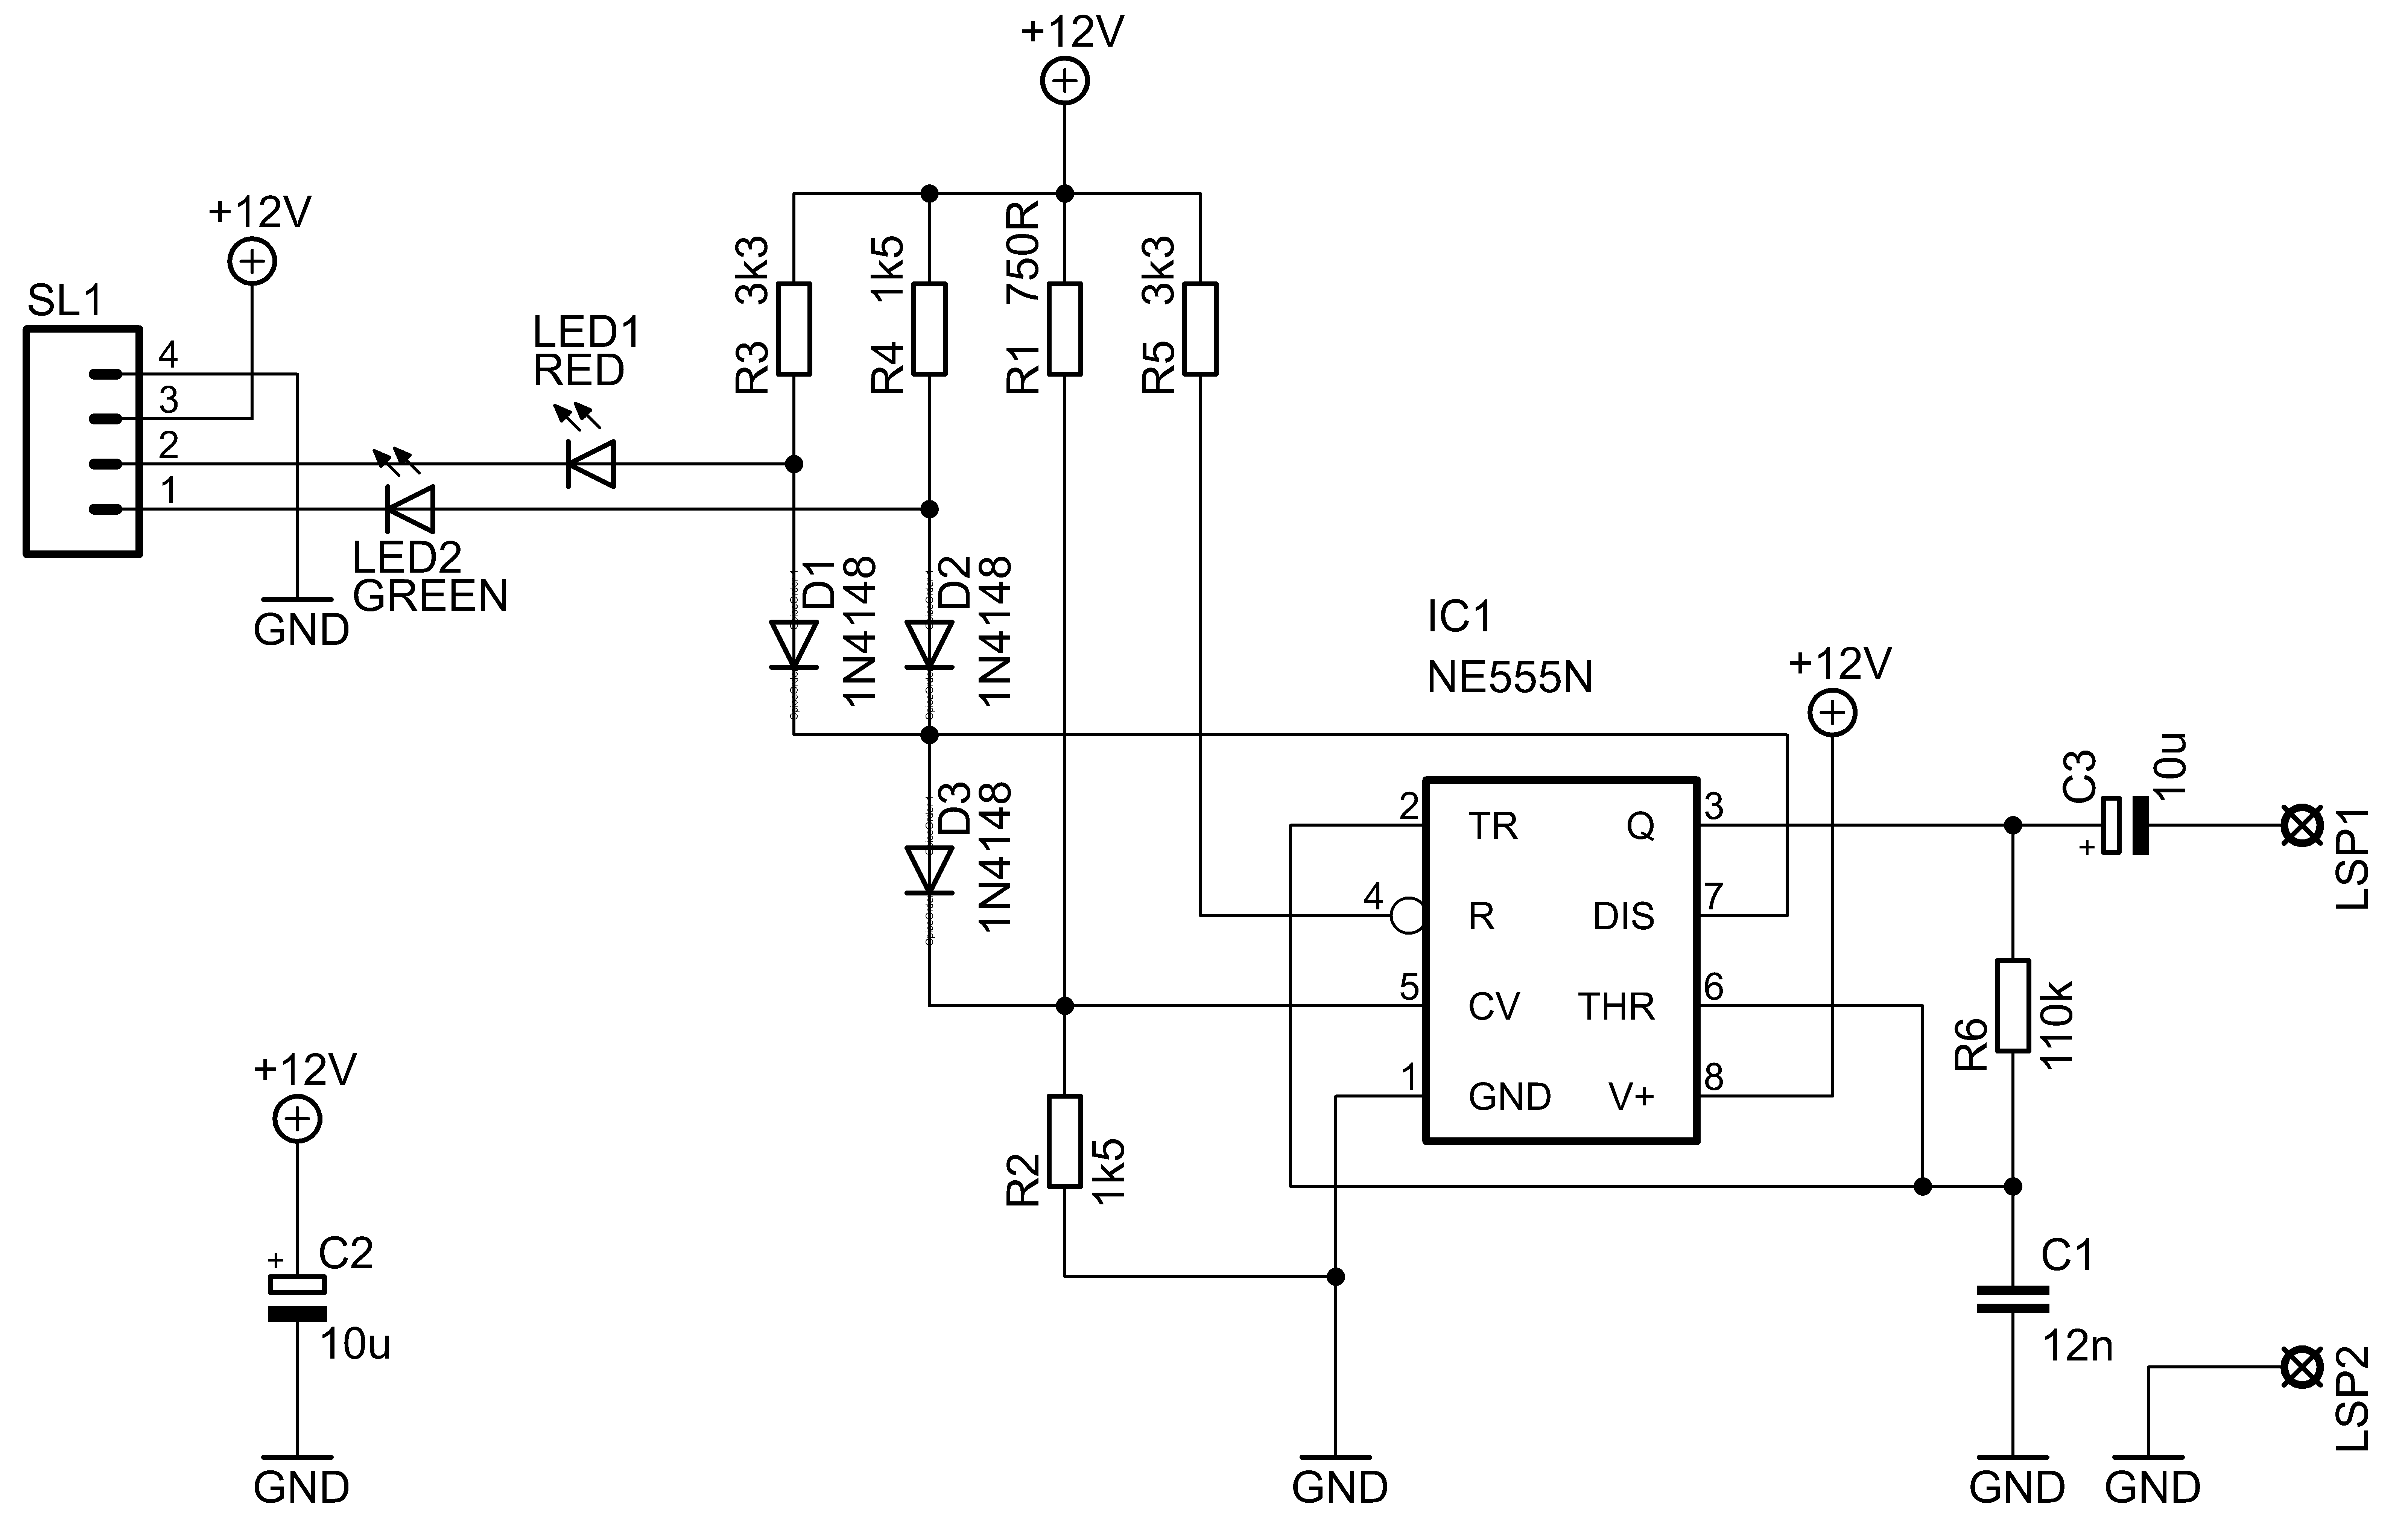
\includegraphics[width=0.8\columnwidth]{osazovani_dps/svetla_piskle_schema}
	\caption{Sch�ma zapojen� signalizace rozsv�cen�ch sv�tel}
  \label{fig:osDPS:schemaZap}
\end{figure}

\begin{figure}[h]
  \centering
  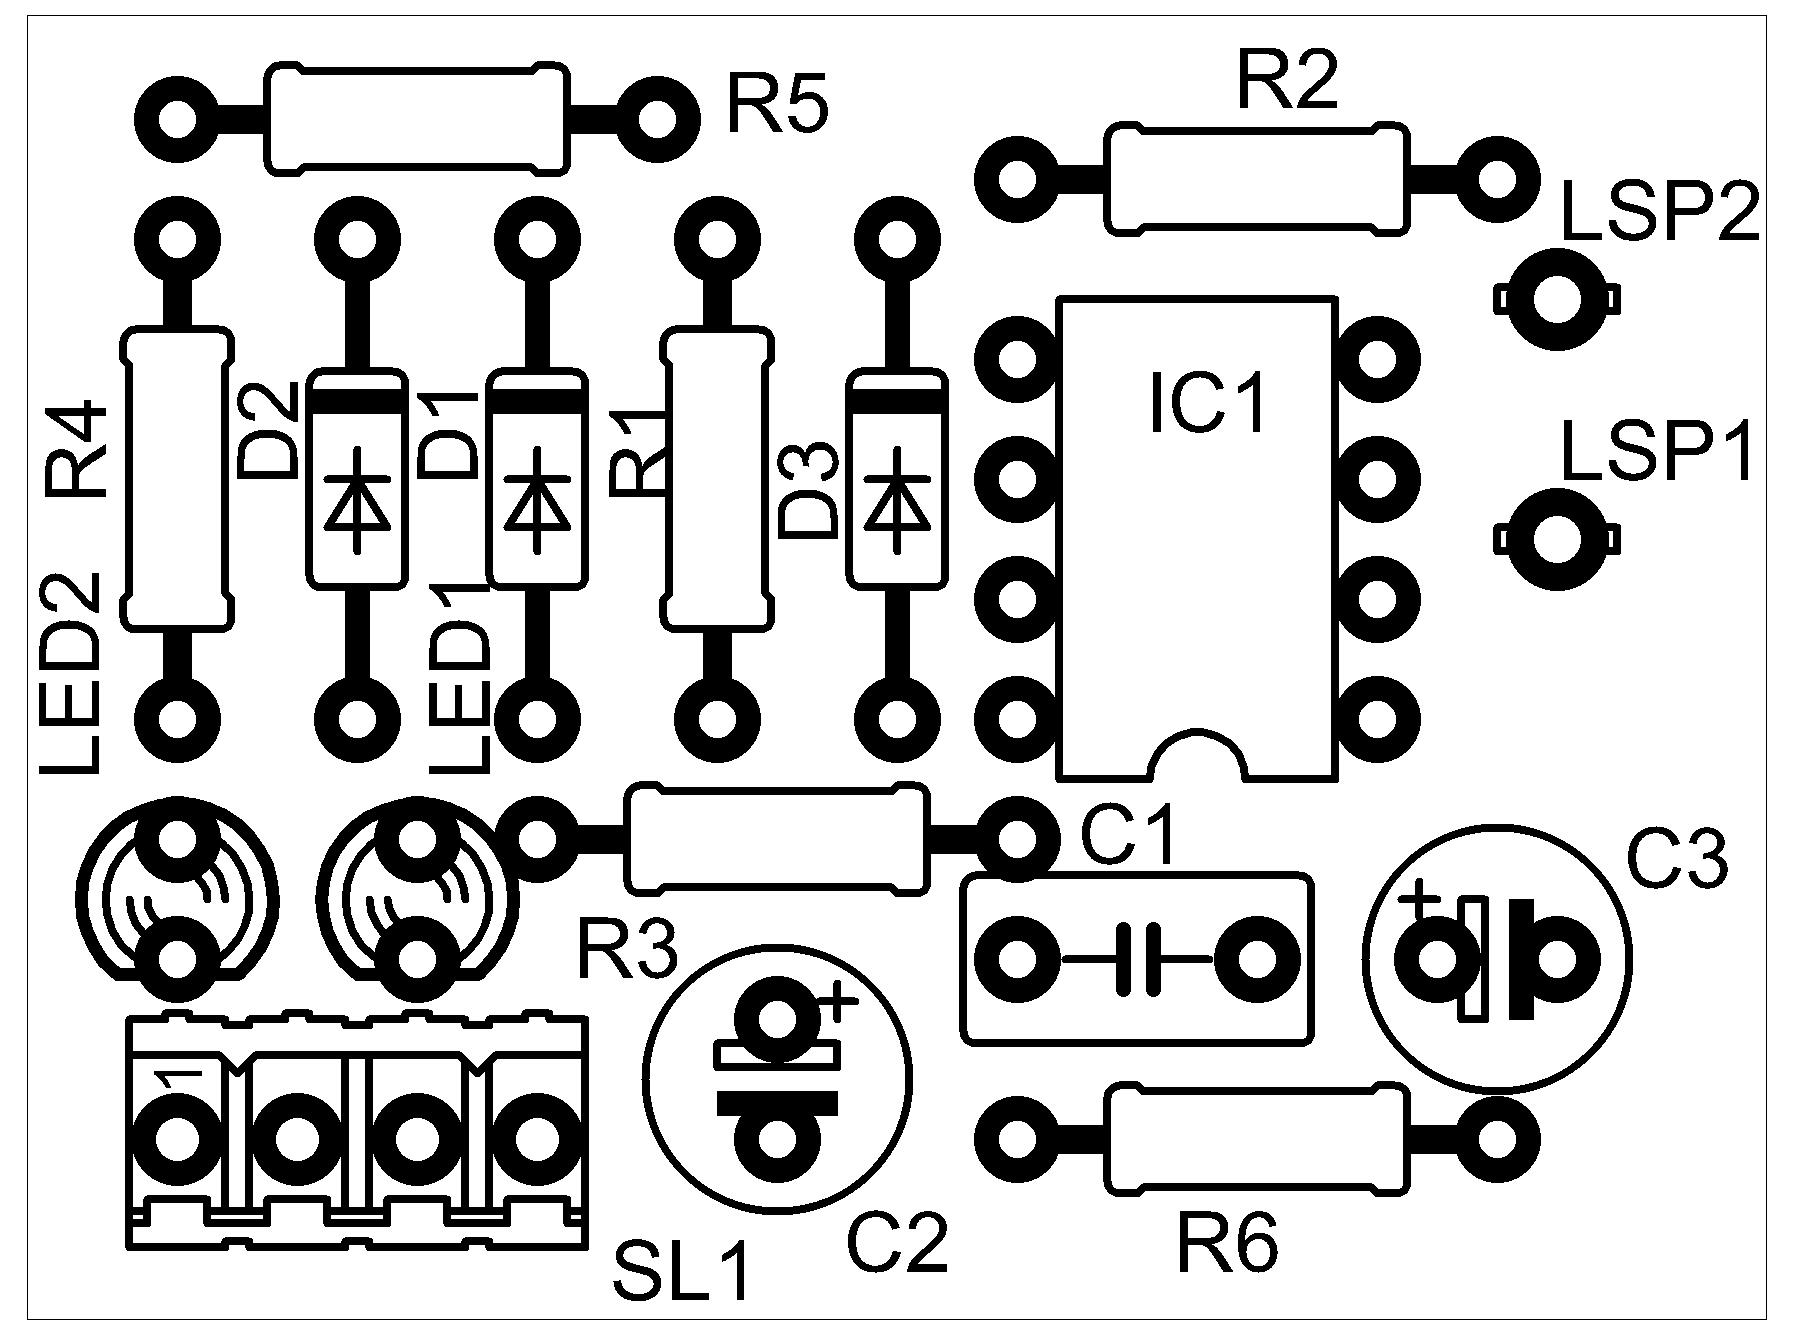
\includegraphics[width=0.4\columnwidth]{osazovani_dps/piskle_S}
	\caption{Pokl�dac� (osazovac�) sch�ma}
  \label{fig:osDPS:schemaPokl}
\end{figure}

\subsubsection{\texorpdfstring{Zna�en� rezistor�}{Znaceni rezistoru}}

\begin{center}
\begin{tabular}{|l|c|c|c|c|c|}
\hline
 Barva & 1. pruh & 2. pruh & 3. pruh & N�sobitel & Tolerance \\
\hline
 �ern� & 0 & 0 & 0 & 1 &\\
 hn�d� & 1 & 1 & 1 & 10 & 1\% \\
 �erven� & 2 & 2 & 2 & 100 & 2\% \\
 oran�ov� & 3 & 3 & 3 & $10^3$ & \\
 �lut� & 4 & 4 & 4 & $10^4$ & \\
 zelen� & 5 & 5 & 5 & $10^5$ & 0,5\% \\
 modr� & 6 & 6 & 6 & $10^6$ & 0,25\%\\
 fialov� & 7 & 7 & 7 & $10^7$ & 0,1\% \\
 �ed� & 8 & 8 & 8 & $10^8$ & 0,05\%\\
 b�l� & 9 & 9 & 9 & $10^9$ & \\
 zlat� &&&& 0,1 & 5\%\\
 st��brn� &&&& 0,01 & 10\%\\
\hline
\end{tabular}
\end{center}

\end{document}
